\section{Results}
\label{sec:results}


The $\jpsi$ and $\psiprime$ non-prompt and prompt production cross-sections are presented, corrected for acceptance and detector efficiencies 
while assuming isotropic decay, as described in Section~\ref{sec:s:diff_xSecDet}. 
Also presented are the ratios of non-prompt production relative to the inclusive production for $\jpsi$ and $\psiprime$ mesons separately, described in Section~\ref{sec:s:NPFDet},
and the ratio of $\psiprime$ to $\jpsi$ production for prompt and non-prompt components separately, described in Section~\ref{sec:s:PNPRatioDet}.
Correction factors for various spin-alignment hypotheses for both 7 and 8~\TeV\  data can be found in 
Tables~\ref{tab:sa_long_jpsi}--\ref{tab:sa_offN_psi2s} (in Appendix) and Tables~\ref{tab:sa_long_jpsi8}--\ref{tab:sa_offN_psi2s8} (in Appendix) respectively, in terms of 
\pt\ and rapidity intervals.

\setdescription{font=\normalfont\itshape}

\begin{description}[style=unboxed,leftmargin=0cm]


\item[Production cross-sections] \hfill

Figures \ref{fig:res:xSecP} and \ref{fig:res:xSecNP} show respectively the prompt and non-prompt 
differential cross-sections of \jpsi\ and \psiprime\ as functions of $\pt$ and $|y|$, together with the relevant theoretical predictions, 
which are described below.


\begin{figure} [!ht]
  \begin{center}
    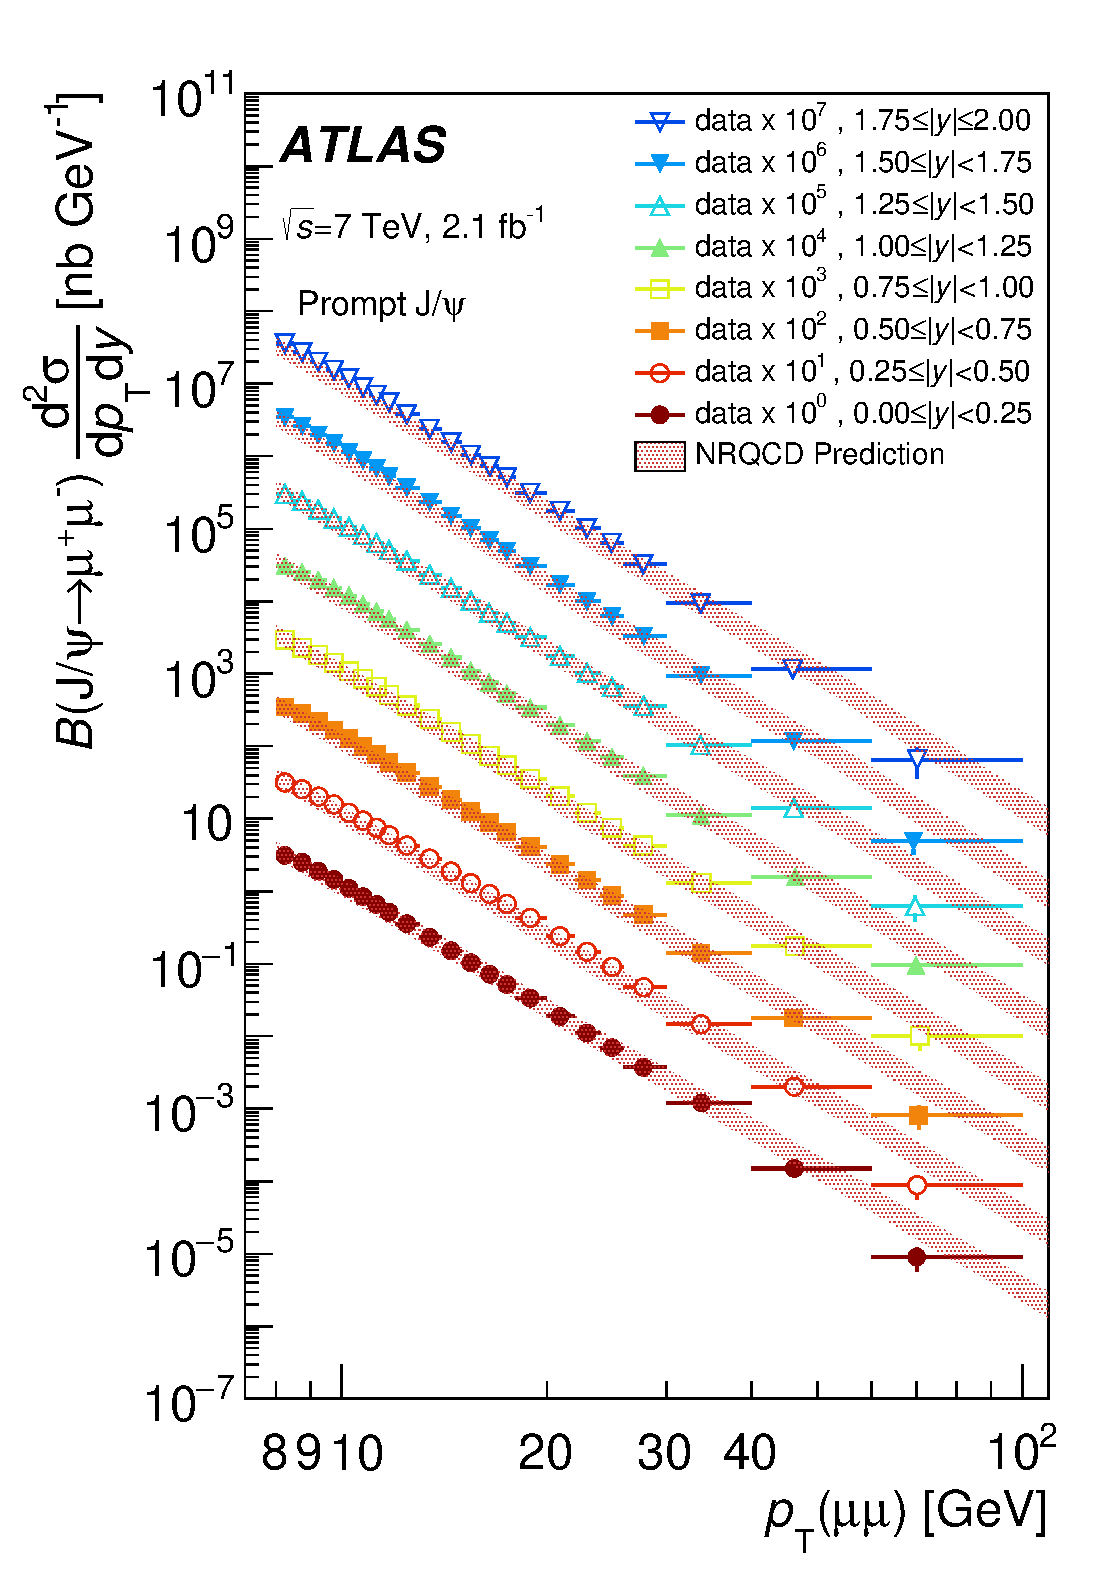
\includegraphics[width=0.44\textwidth]{figures/ct_7TeV_JpsiP_xSec.eps} 
    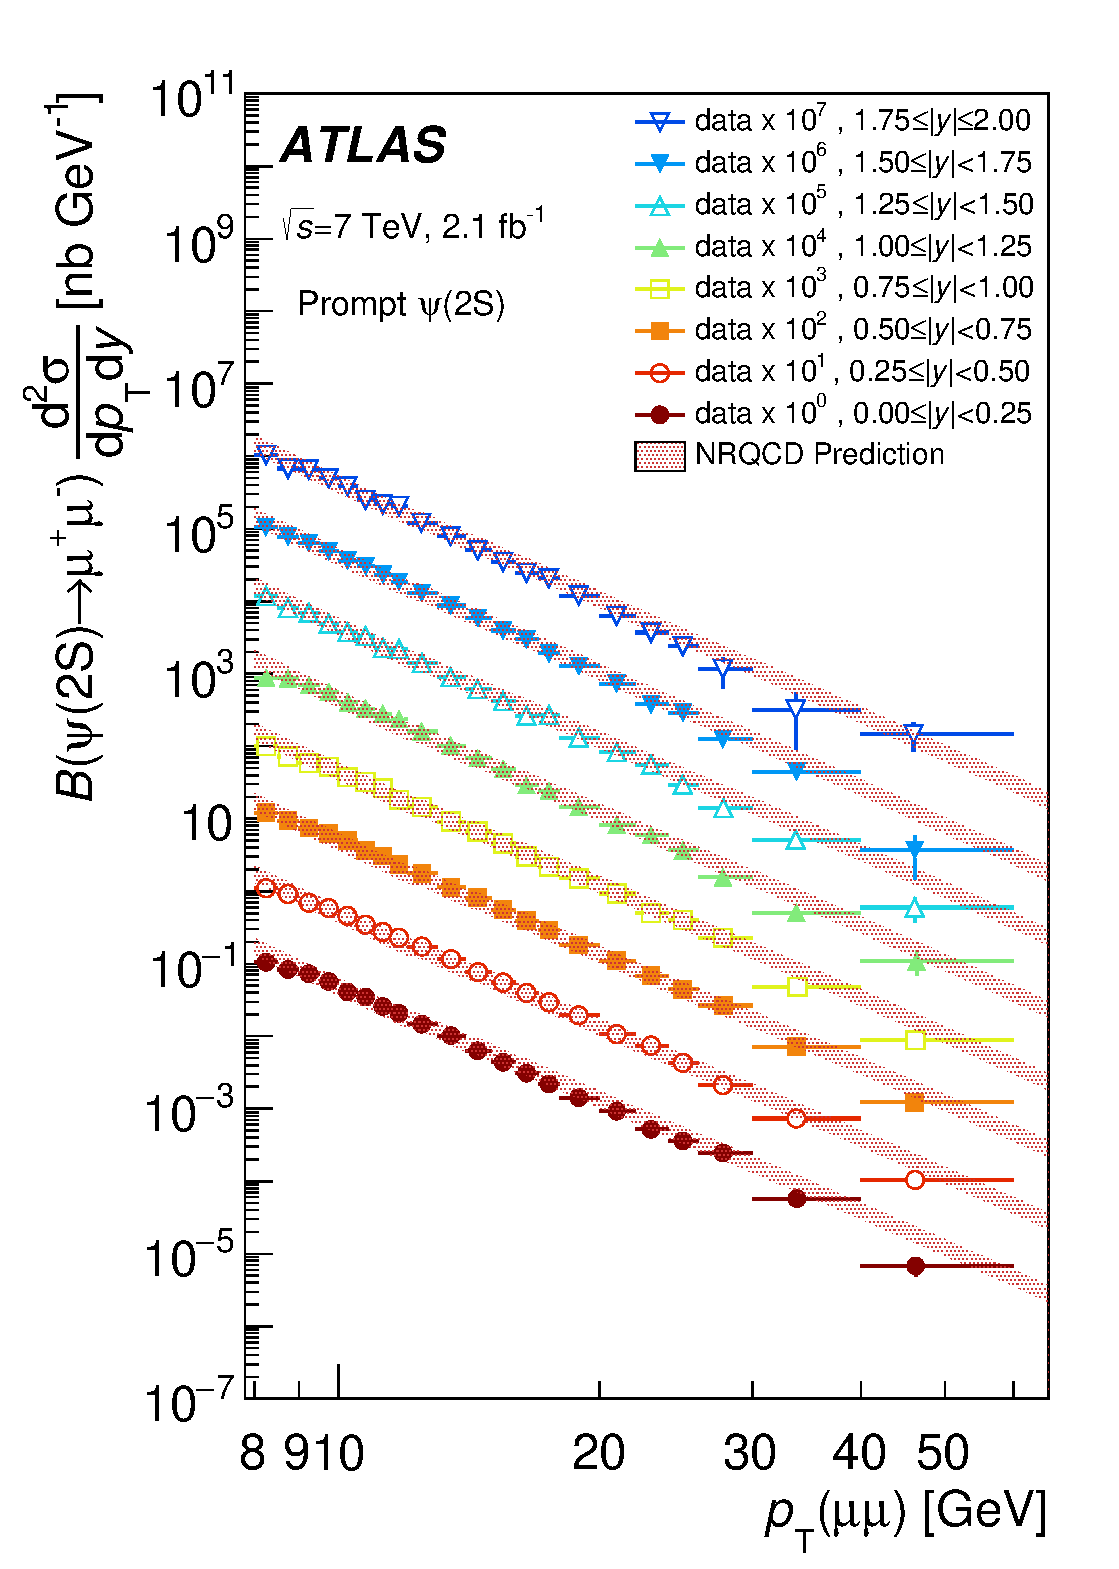
\includegraphics[width=0.44\textwidth]{figures/ct_7TeV_Psi2SP_xSec.eps}\hfil\\
    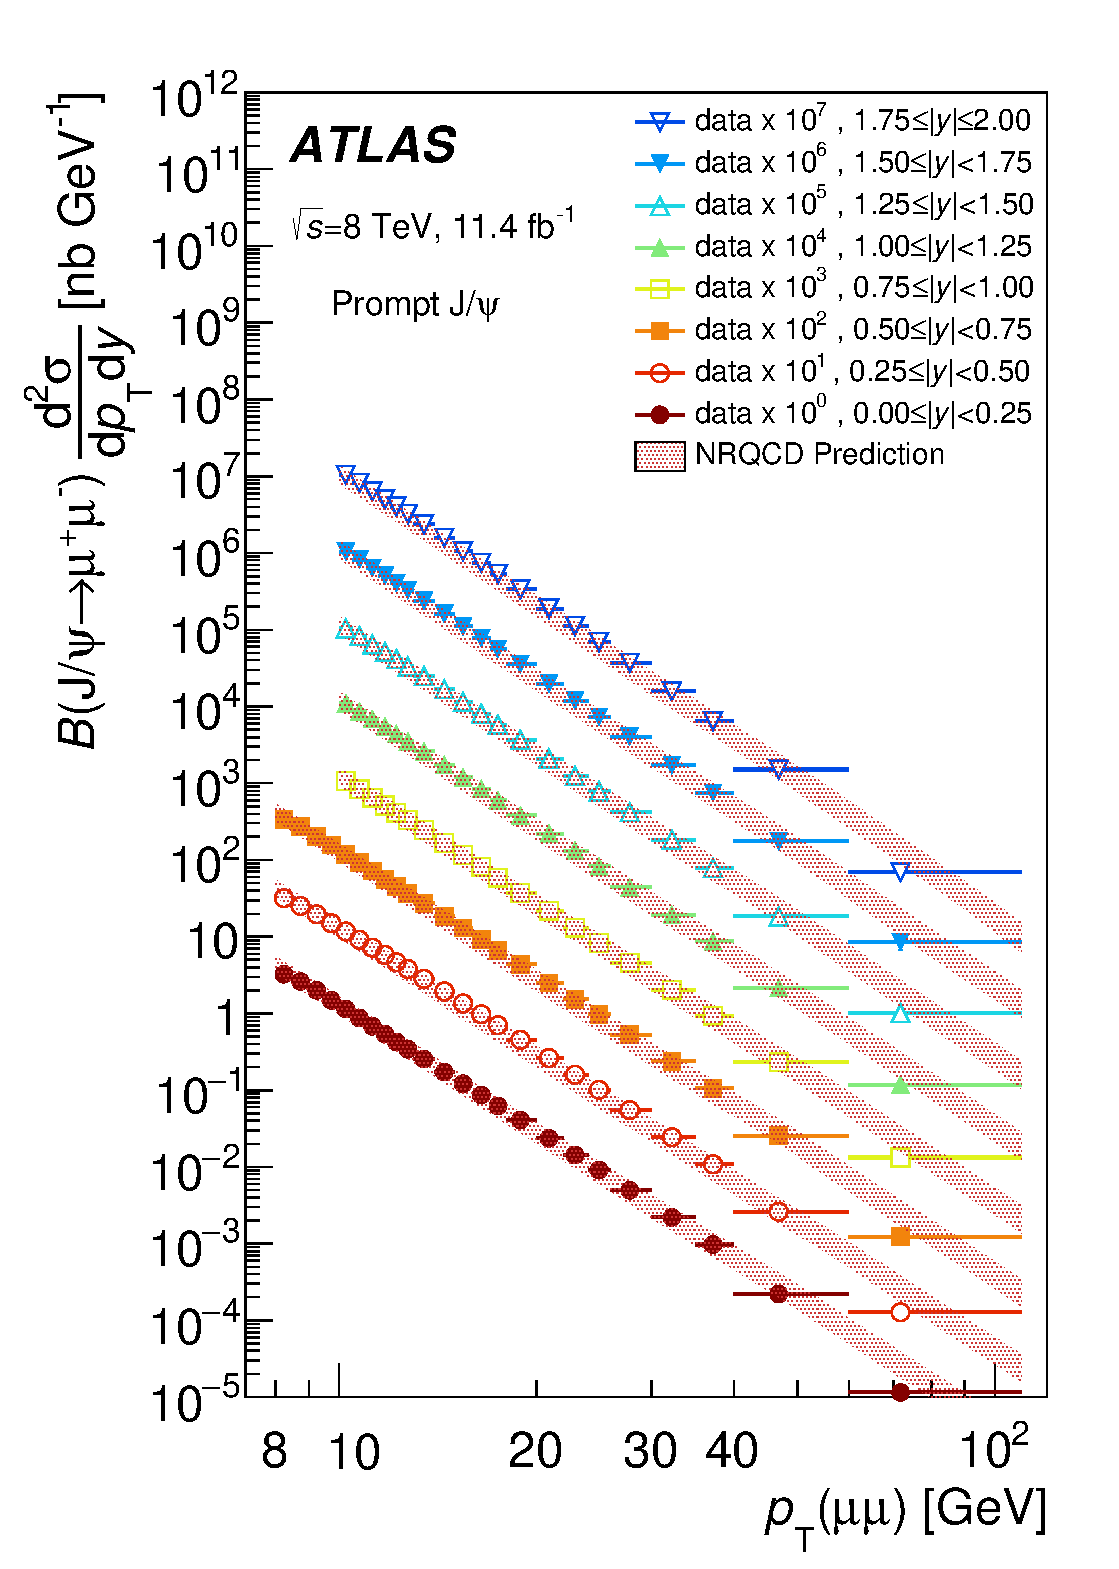
\includegraphics[width=0.44\textwidth]{figures/ct_8TeV_JpsiP_xSec.eps}
    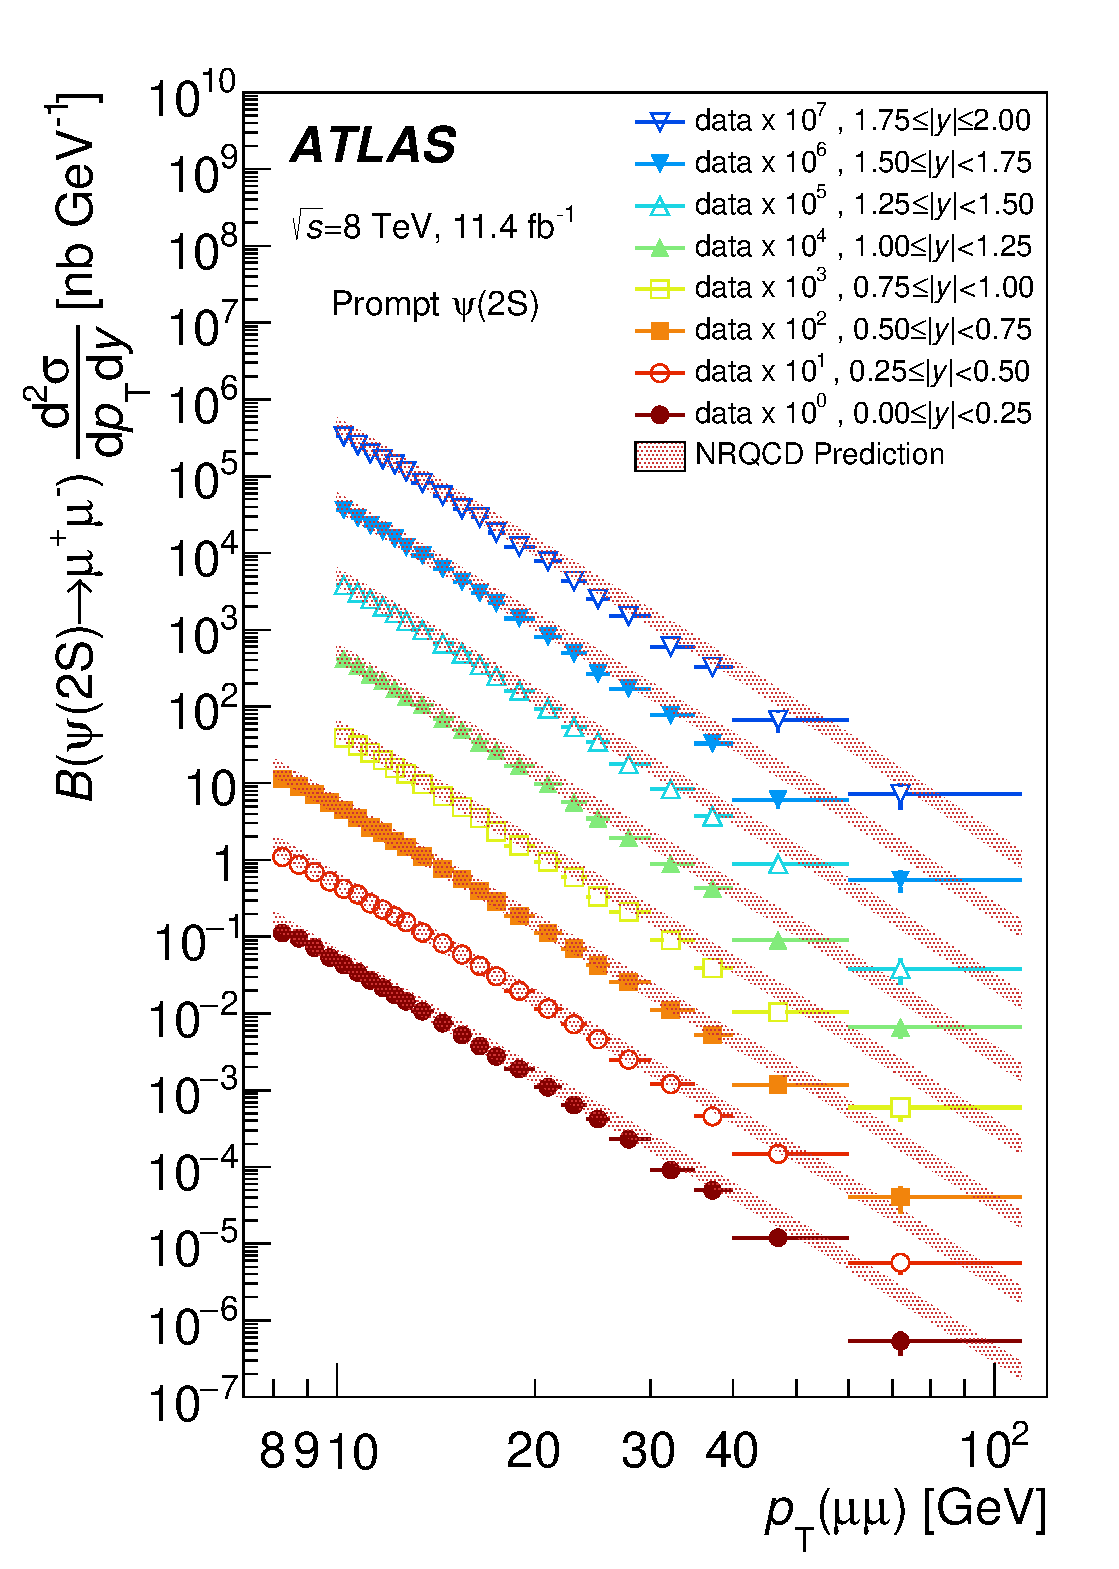
\includegraphics[width=0.44\textwidth]{figures/ct_8TeV_Psi2SP_xSec.eps}\hfil
    \caption{The differential prompt cross-section times dimuon branching fraction of \jpsi\ (left) and \psiprime\ (right) as a function 
    of $\pt(\mu\mu)$ for each slice of rapidity. 
    The top (bottom) row shows the 7~\TeV\ (8~\TeV) results.
    For each increasing rapidity slice, an additional scaling factor of 10 is applied to the plotted points for visual clarity. The
      centre of each bin on the horizontal axis represents the mean of the weighted $\pt$ distribution. The
      horizontal error bars represent the range of $\pt$ for the bin, and the vertical error bar covers 
      the statistical and systematic 
      uncertainty (with the same multiplicative scaling applied). 
      The NLO NRQCD theory predictions are also shown.}
    \label{fig:res:xSecP}
  \end{center}
\end{figure} 

\begin{figure} [!ht]
  \begin{center} 
    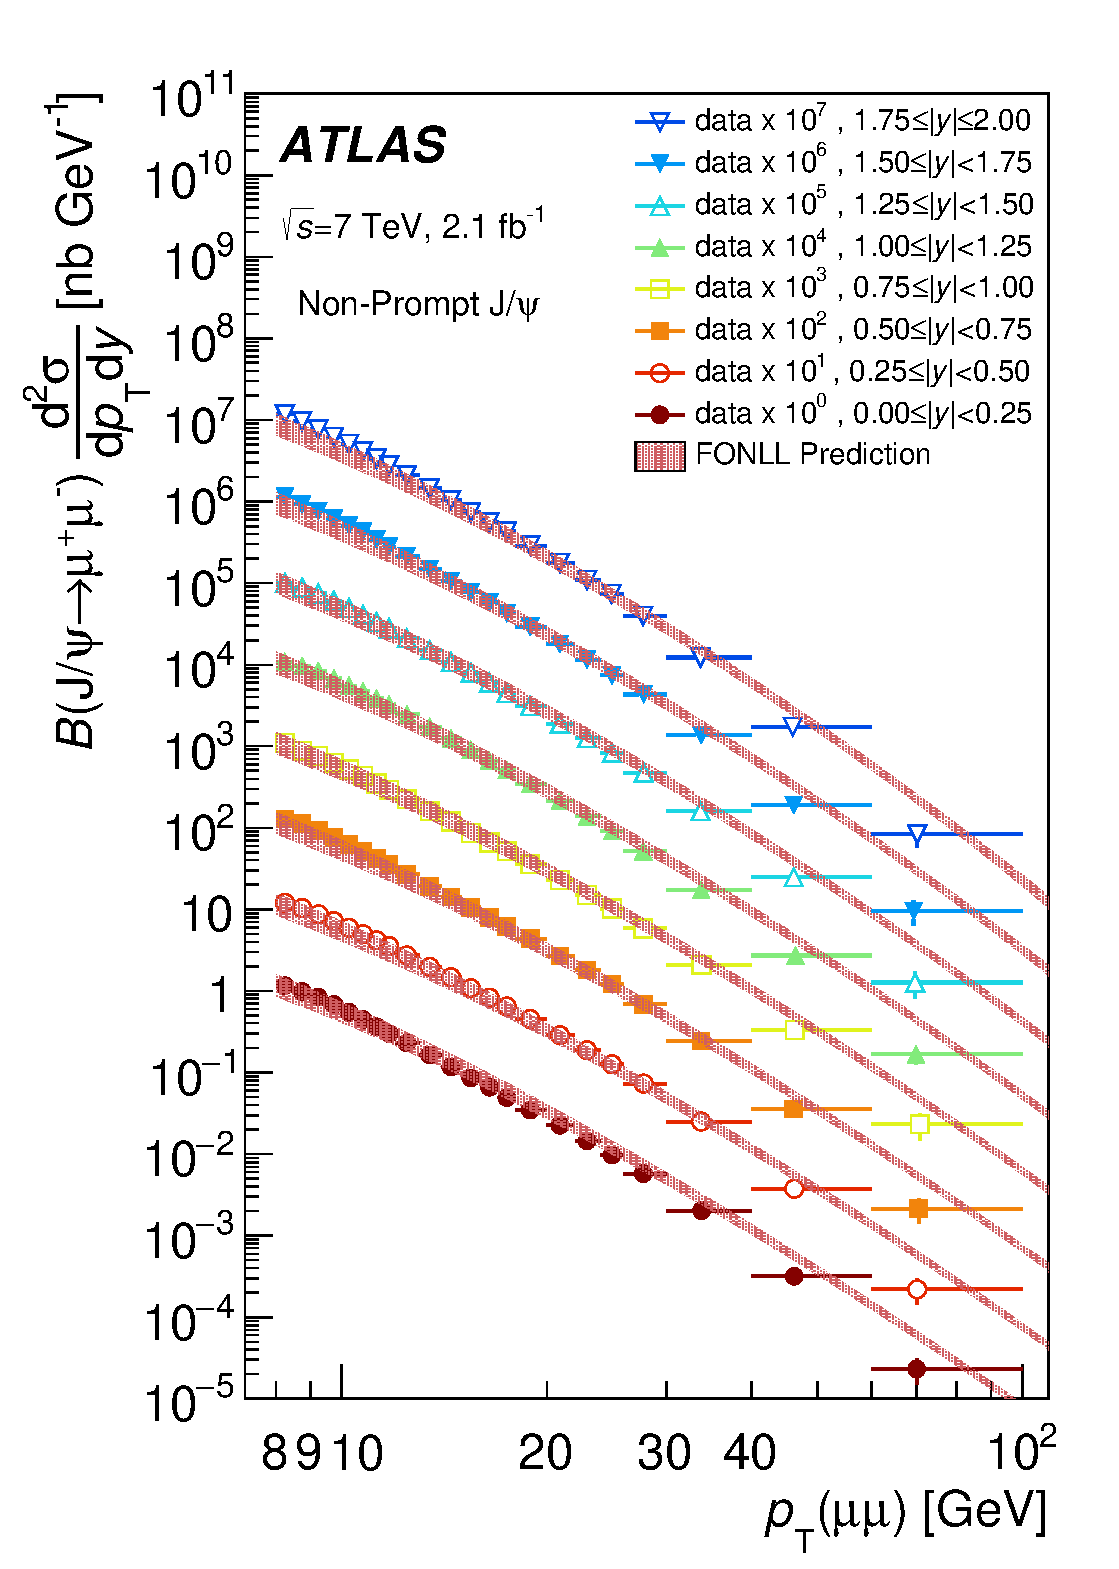
\includegraphics[width=0.44\textwidth]{figures/ct_7TeV_JpsiNP_xSec.eps}
    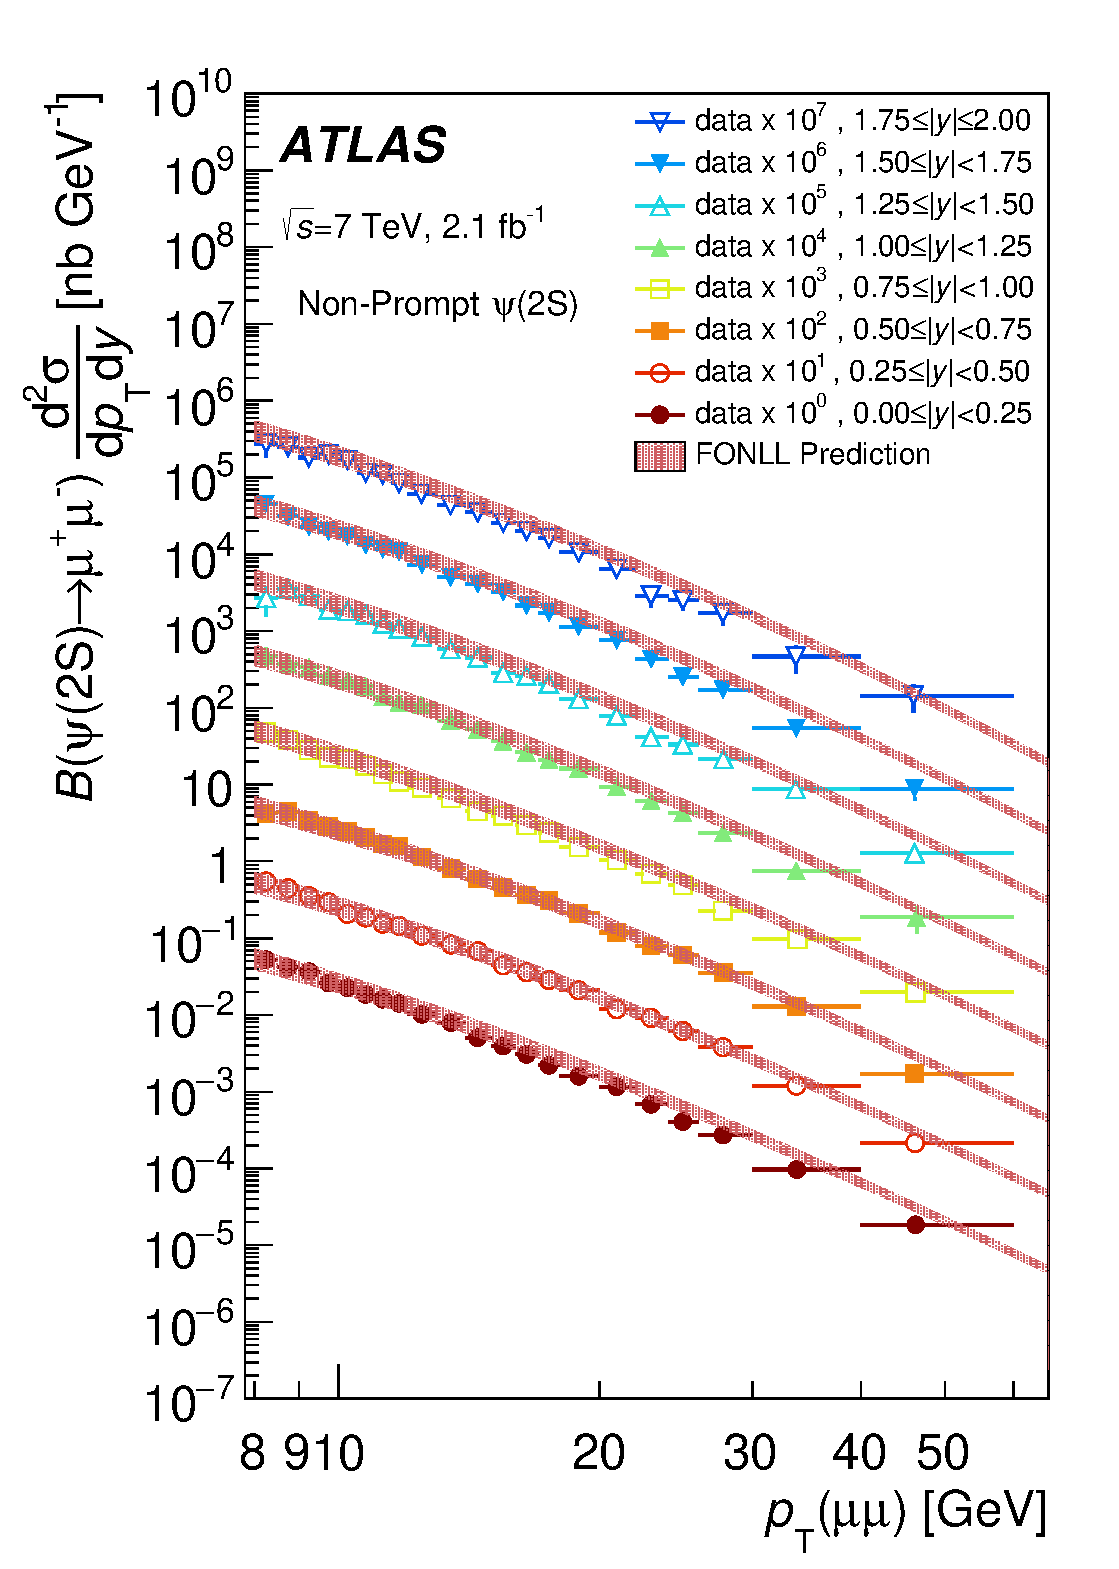
\includegraphics[width=0.44\textwidth]{figures/ct_7TeV_Psi2SNP_xSec.eps}\hfil
    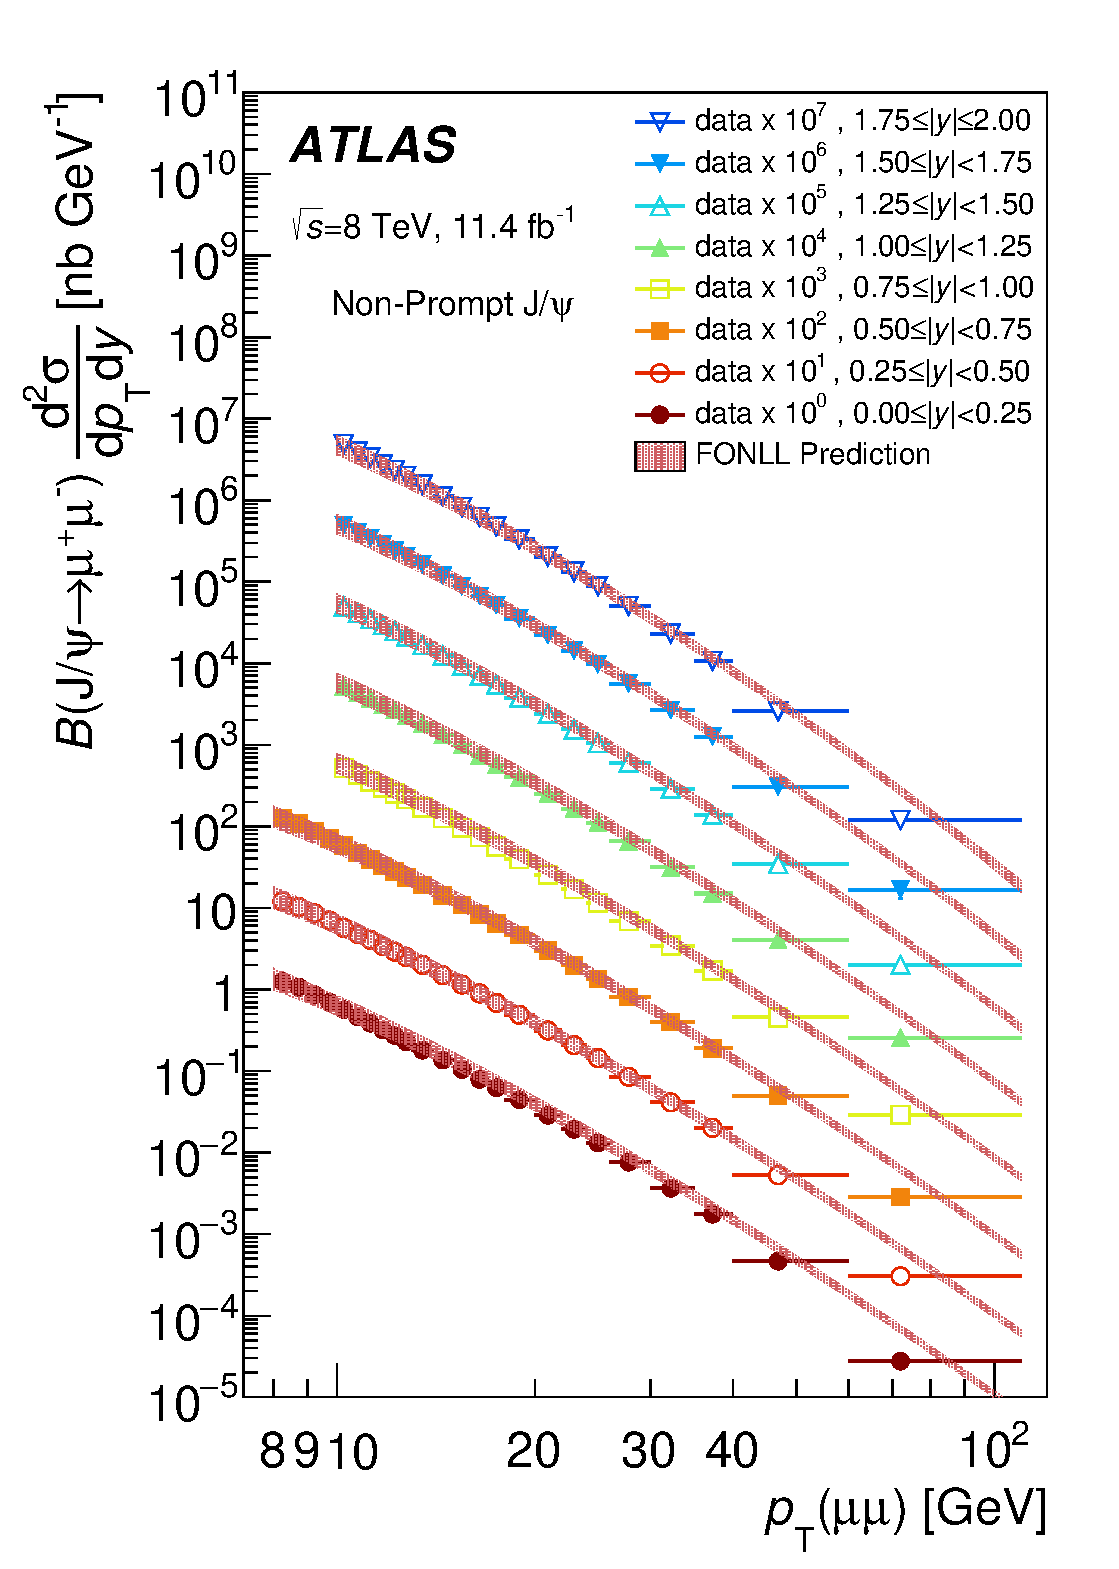
\includegraphics[width=0.44\textwidth]{figures/ct_8TeV_JpsiNP_xSec.eps}
    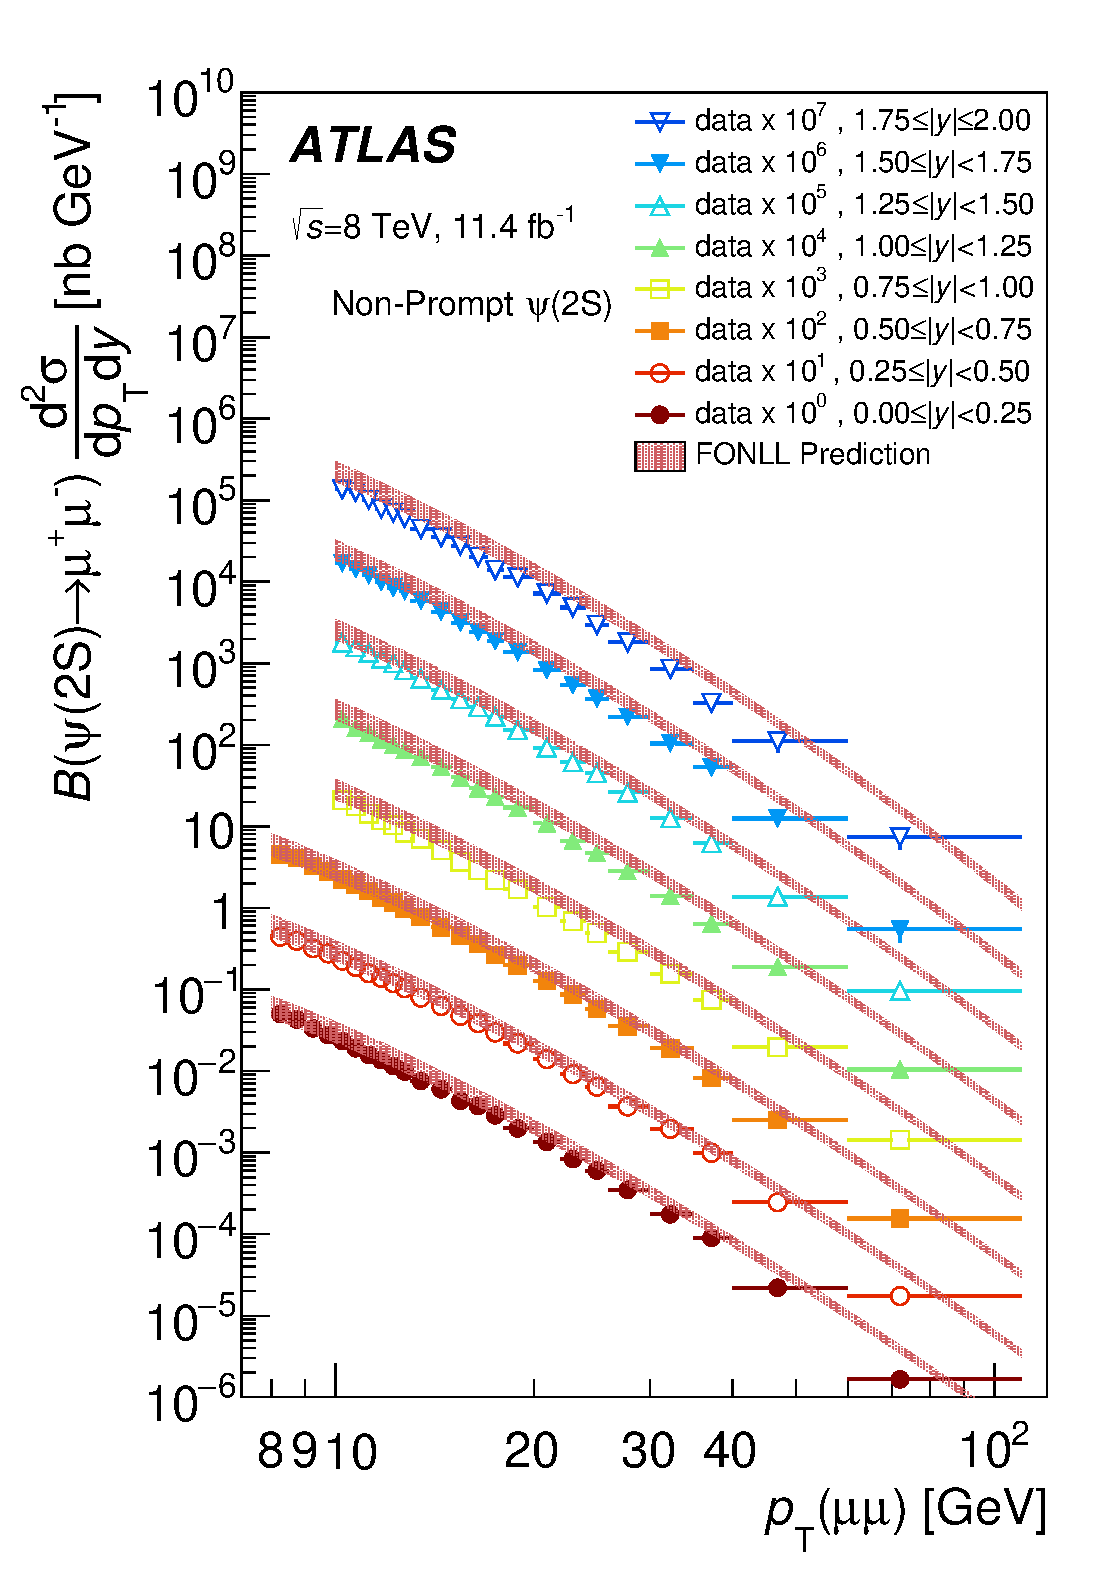
\includegraphics[width=0.44\textwidth]{figures/ct_8TeV_Psi2SNP_xSec.eps}\hfil
    \caption{The differential non-prompt cross-section times dimuon branching fraction of \jpsi\ (left) and \psiprime\ (right) as a function 
    of $\pt(\mu\mu)$ for each slice of rapidity. 
    The top (bottom) row shows the 7~\TeV\ (8~\TeV) results.
    For each increasing rapidity slice, an additional scaling factor of 10 is applied to the plotted points for visual clarity. The
      centre of each bin on the horizontal axis represents the mean of the weighted $\pt$ distribution. The
      horizontal error bars represent the range of $\pt$ for the bin, and the vertical error bar covers the statistical
      and systematic uncertainty (with the same multiplicative scaling applied).
      The FONLL theory predictions are also shown.}
    \label{fig:res:xSecNP}
  \end{center}
\end{figure} 


\item[Non-prompt production fractions] \hfill % \\

The results for the fractions of non-prompt production relative to the inclusive production of \jpsi\ and \psiprime\, are presented as a function of $\pt$ for slices of rapidity in Figure~\ref{fig:res:NPF}. 
In each rapidity slice, the non-prompt fraction is seen to increase as a function of $\pt$ and has no strong dependence on either rapidity or centre-of-mass energy.

\begin{figure} [!ht]
  \begin{center}
    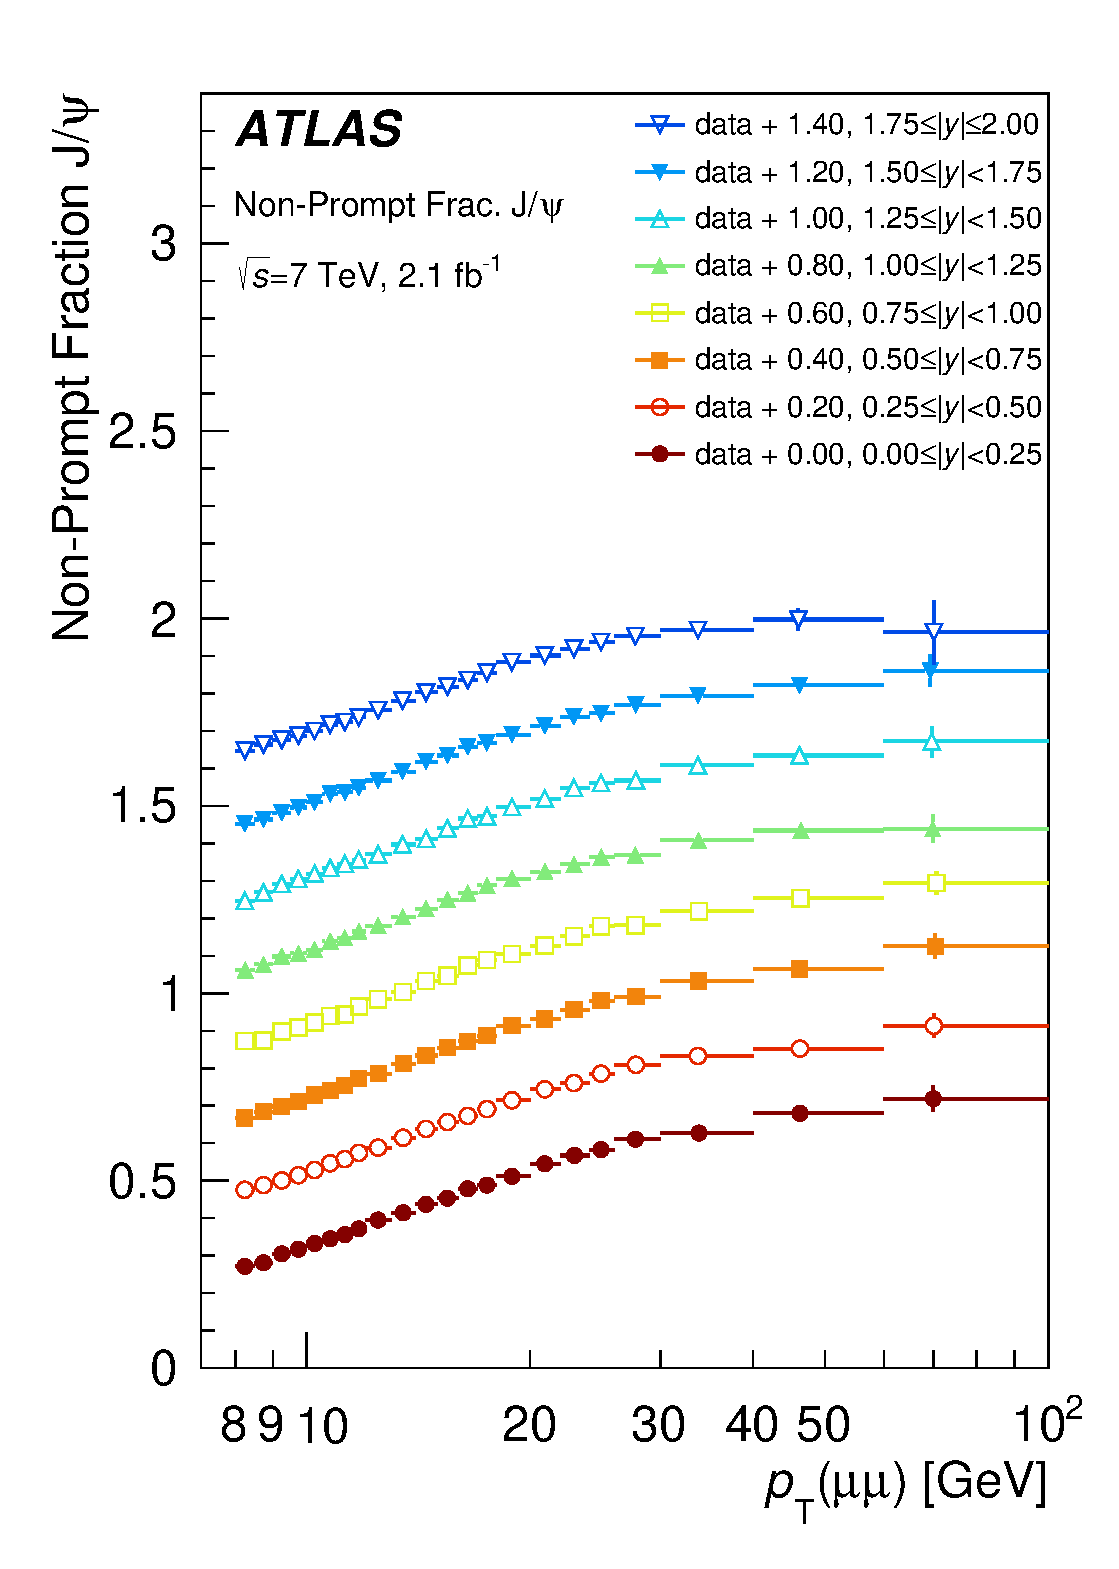
\includegraphics[width=0.44\textwidth]{figures/ct_7TeV_NPF_Jpsi.eps} 
    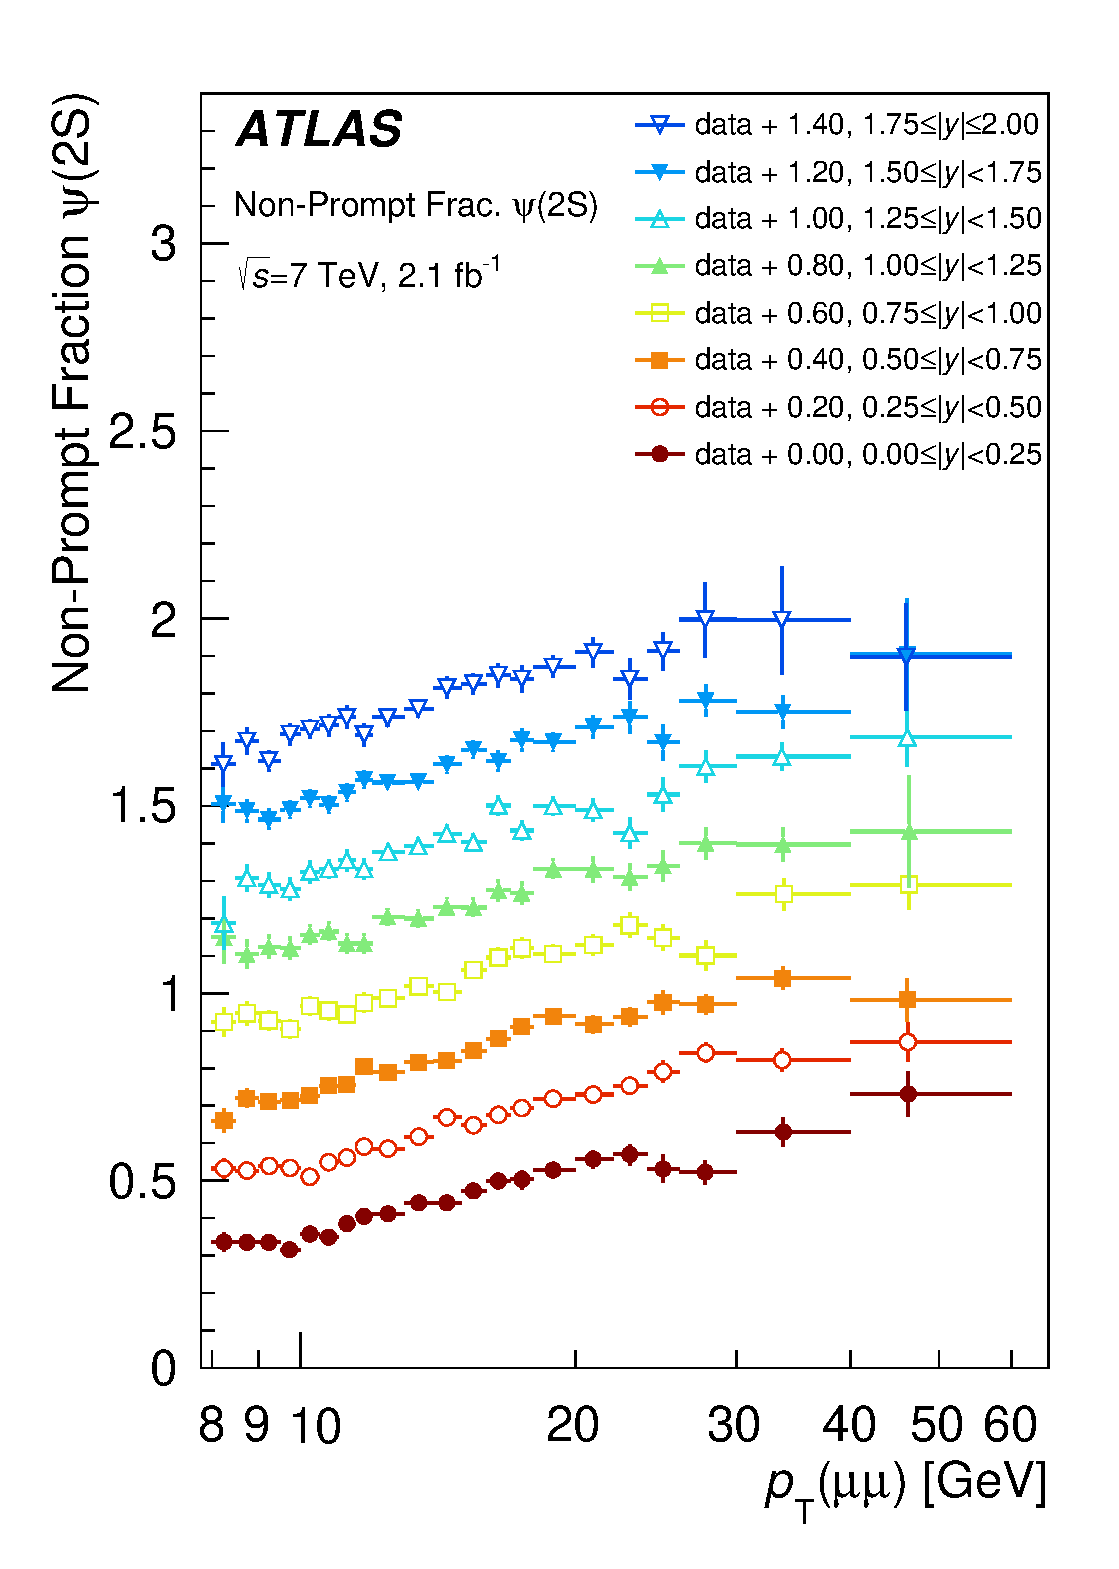
\includegraphics[width=0.44\textwidth]{figures/ct_7TeV_NPF_Psi.eps}\hfil\\
    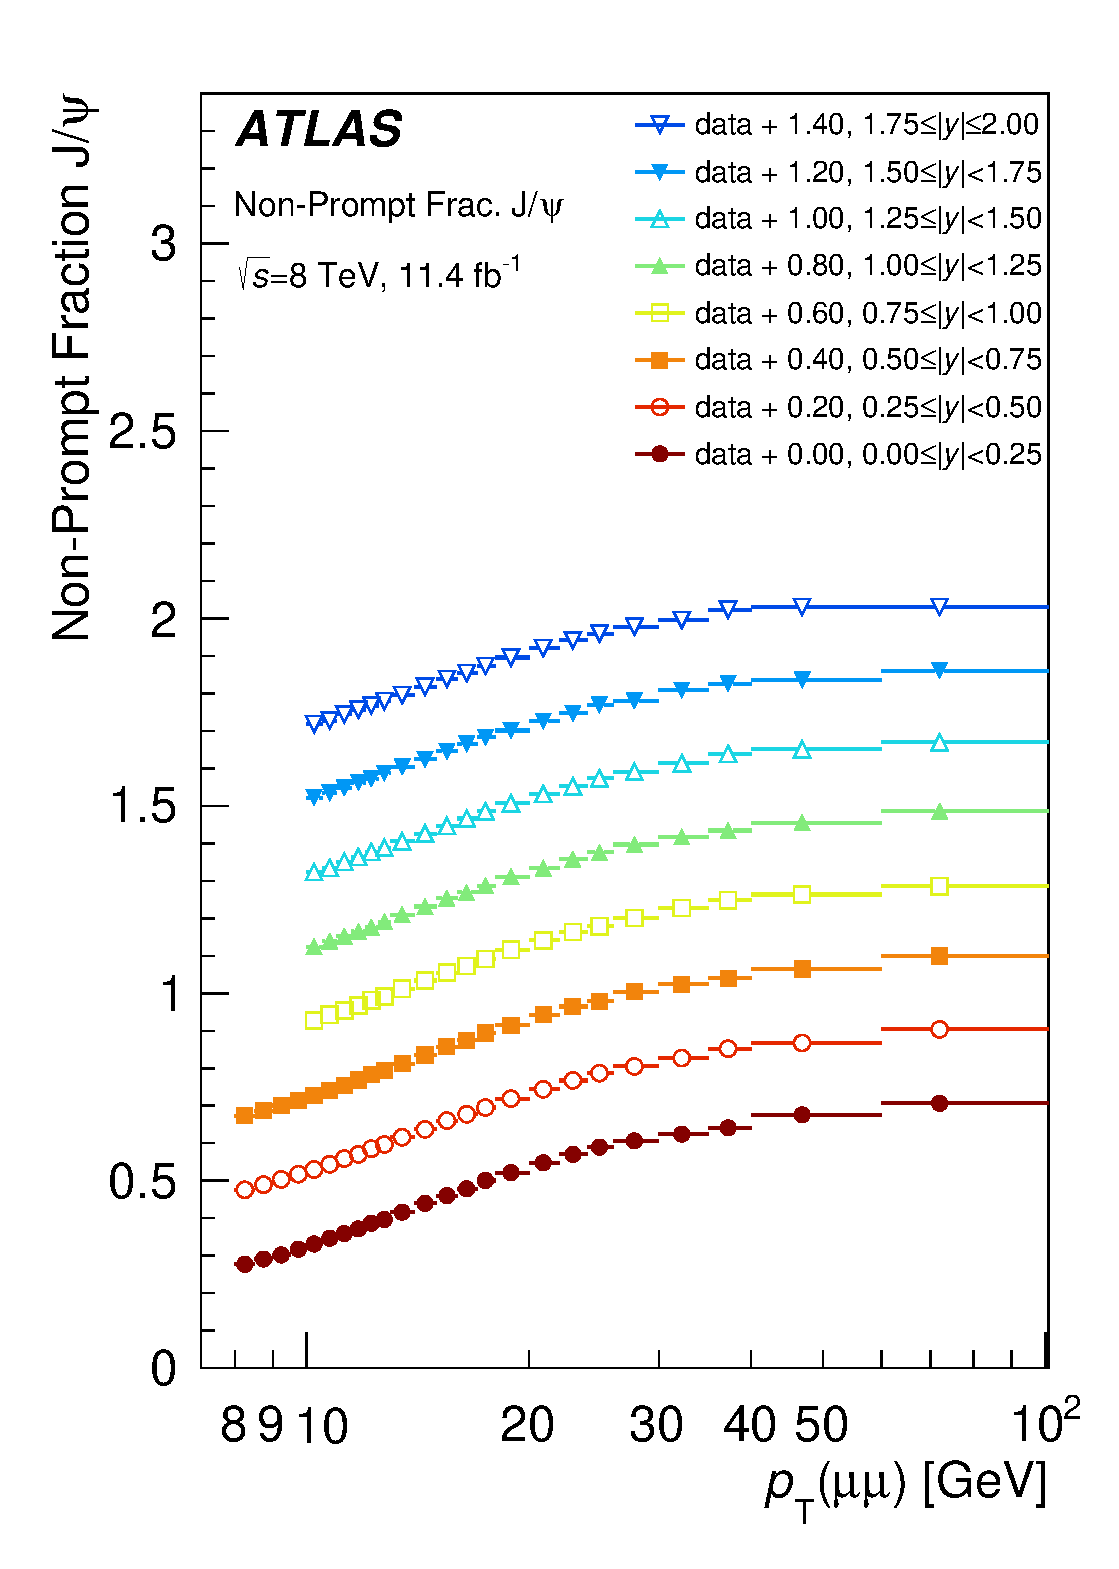
\includegraphics[width=0.44\textwidth]{figures/ct_8TeV_NPF_Jpsi.eps}
    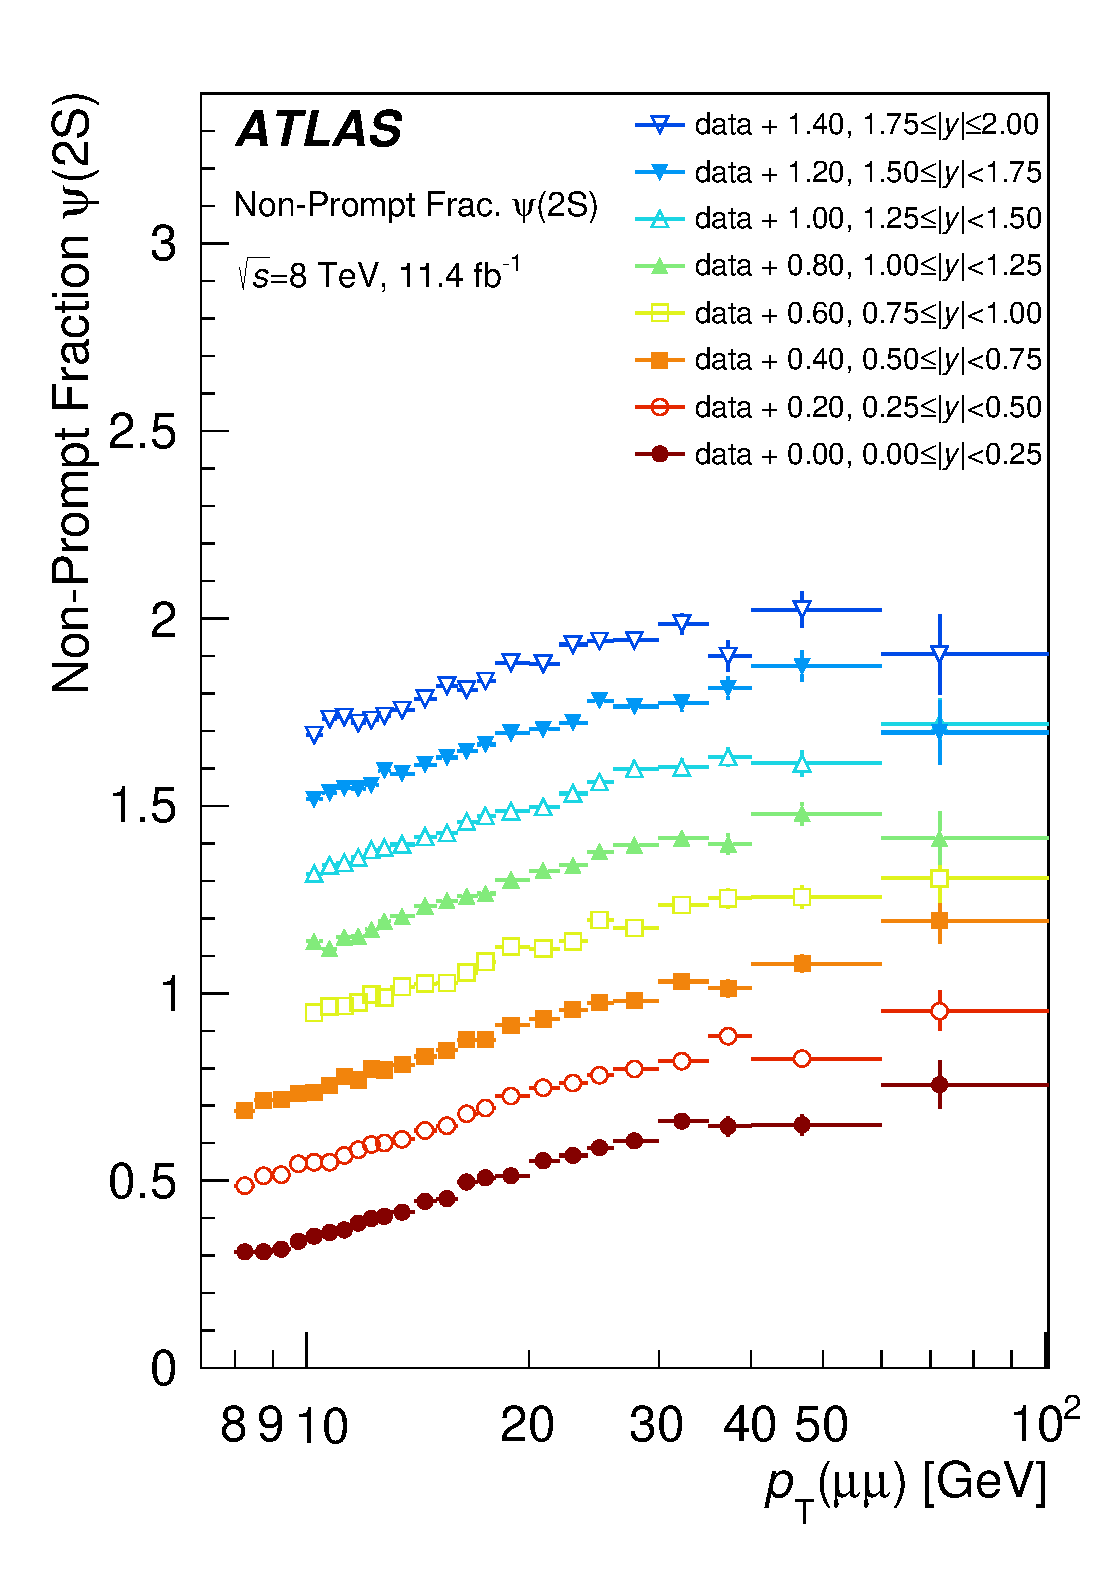
\includegraphics[width=0.44\textwidth]{figures/ct_8TeV_NPF_Psi.eps}\hfil
    \caption{The non-prompt fraction of \jpsi\ (left) and \psiprime\ (right), as a function of $\pt(\mu\mu)$ for each slice of rapidity. 
    The top (bottom) row shows the 7~\TeV\ (8~\TeV) results.
      For each increasing rapidity slice, an additional factor of 0.2 is applied to the plotted points for visual clarity. The
      centre of each bin on the horizontal axis represents the mean of the weighted $\pt$ distribution. The
      horizontal error bars represent the range of $\pt$ for the bin, and the vertical error bar covers the statistical
    and systematic  uncertainty (with the same multiplicative scaling applied).}
    \label{fig:res:NPF}
  \end{center}
\end{figure} 


\textit{Production ratios of \textmd{\psiprime} to \textmd{\jpsi} }

Figure~\ref{fig:res:PNP_Ratio} shows the ratios of \psiprime\ to \jpsi\ decaying to a muon pair in prompt and non-prompt processes,
 presented as a function of $\pt$ for slices of rapidity. The non-prompt ratio is shown to be relatively flat across the considered range of $\pT$,
for each slice of rapidity.
For the prompt ratio, a slight increase as a function of $\pt$ is observed, with no strong dependence on rapidity or centre-of-mass energy.

\begin{figure} [!ht]
  \begin{center}
    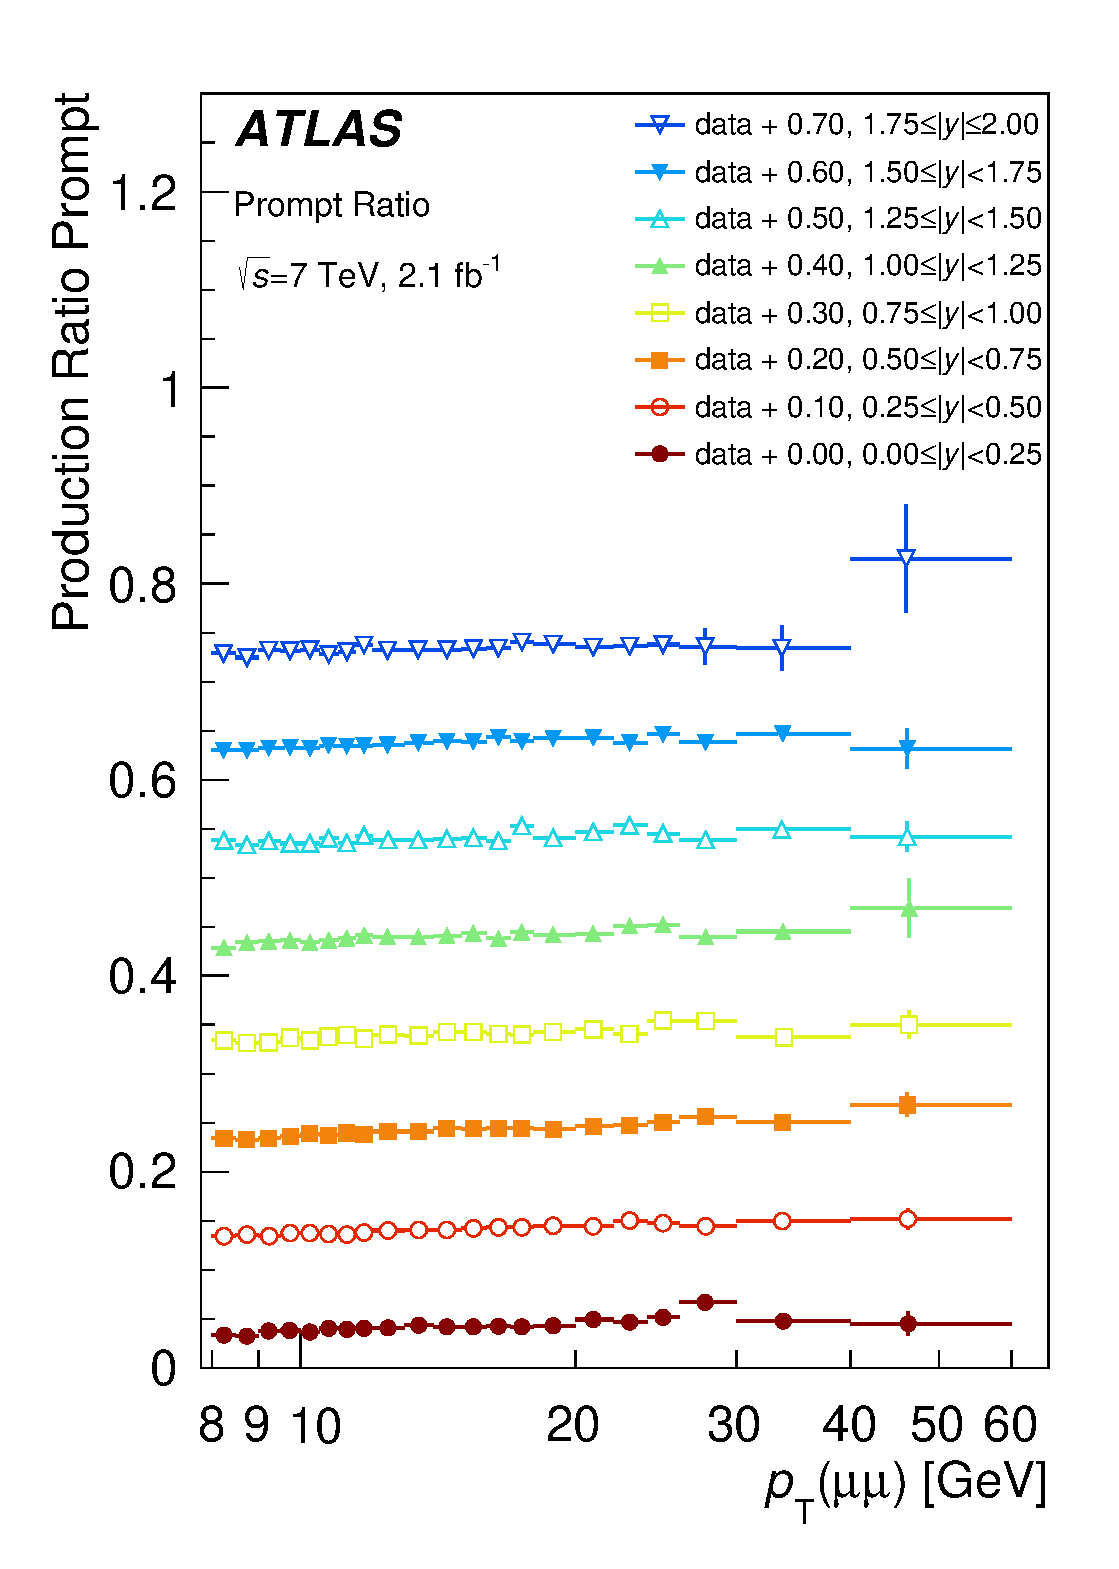
\includegraphics[width=0.44\textwidth]{figures/ct_7TeV_P_Ratio.eps} 
    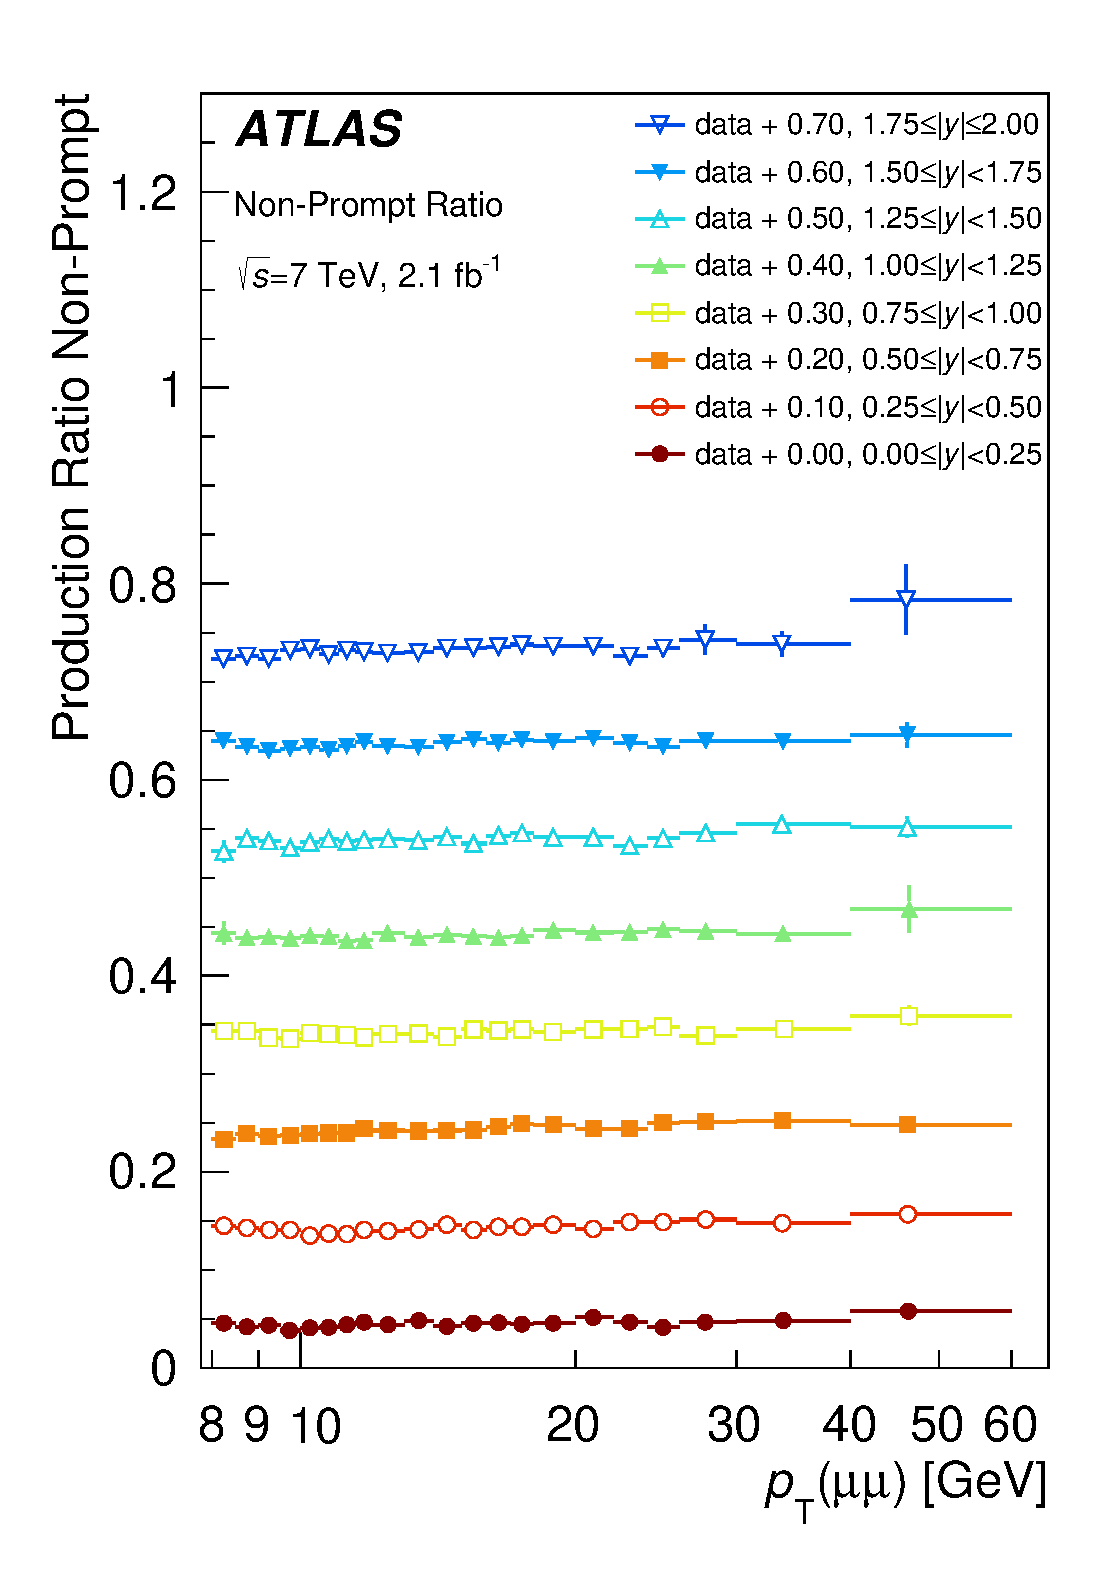
\includegraphics[width=0.44\textwidth]{figures/ct_7TeV_NP_Ratio.eps}\hfil\\
    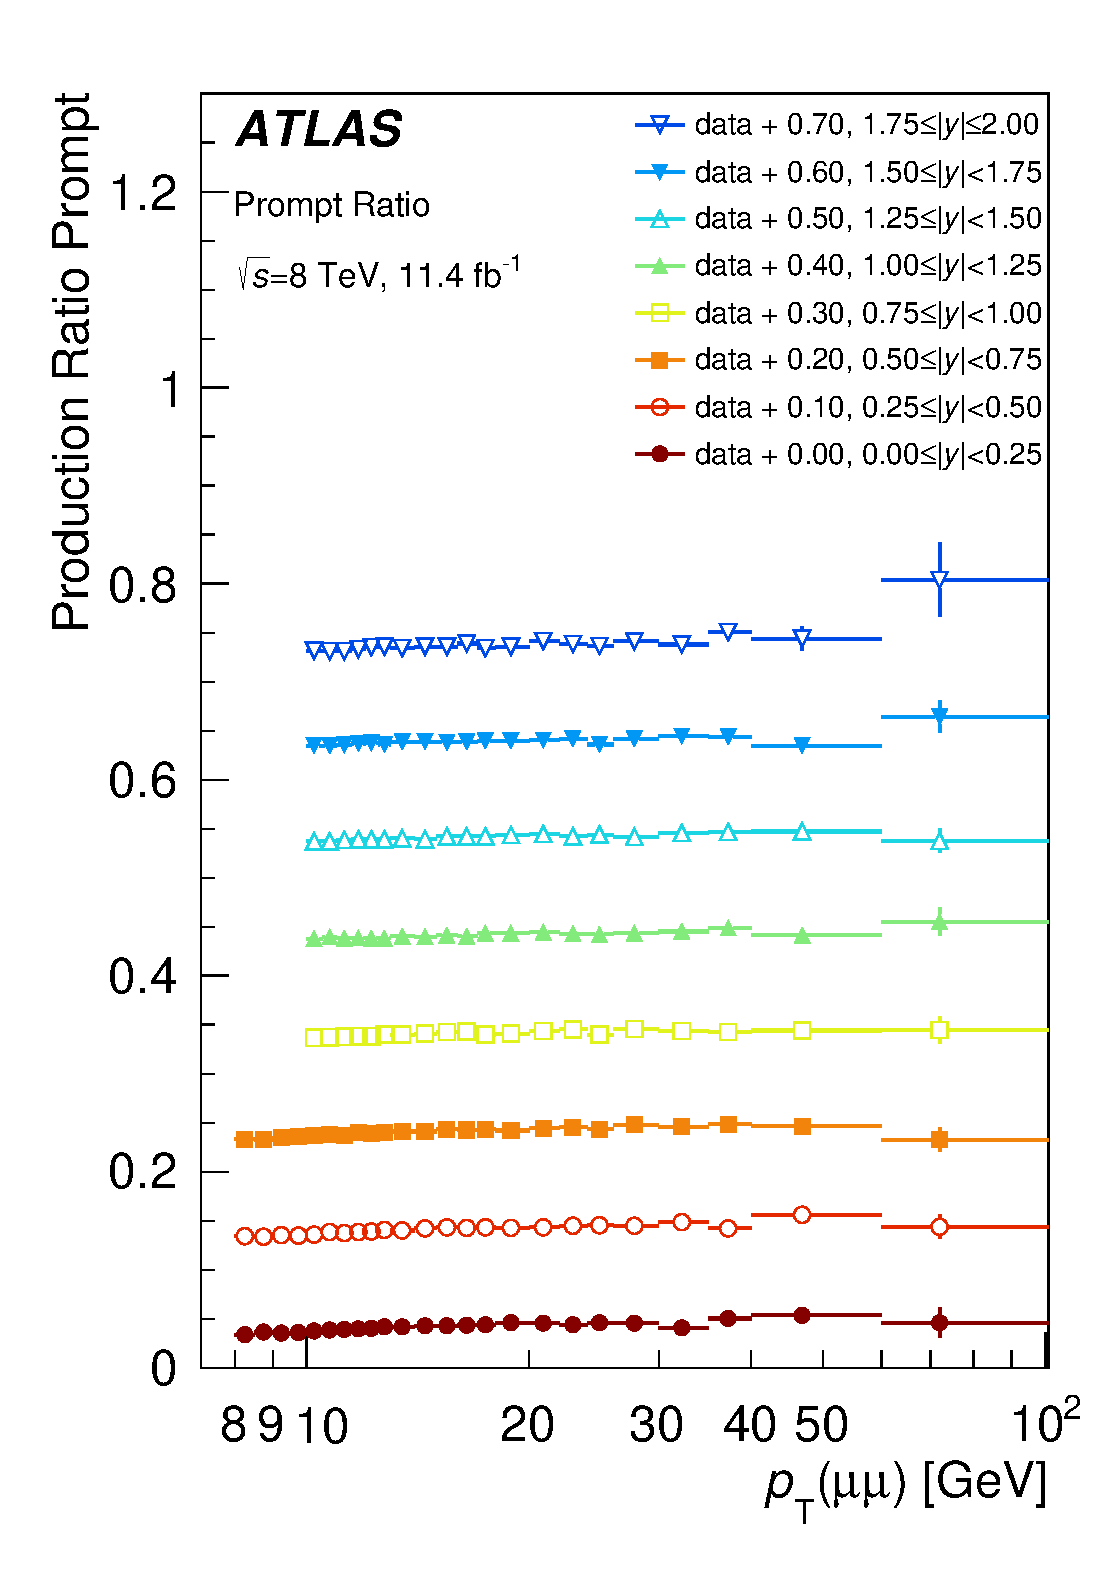
\includegraphics[width=0.44\textwidth]{figures/ct_8TeV_P_Ratio.eps}
    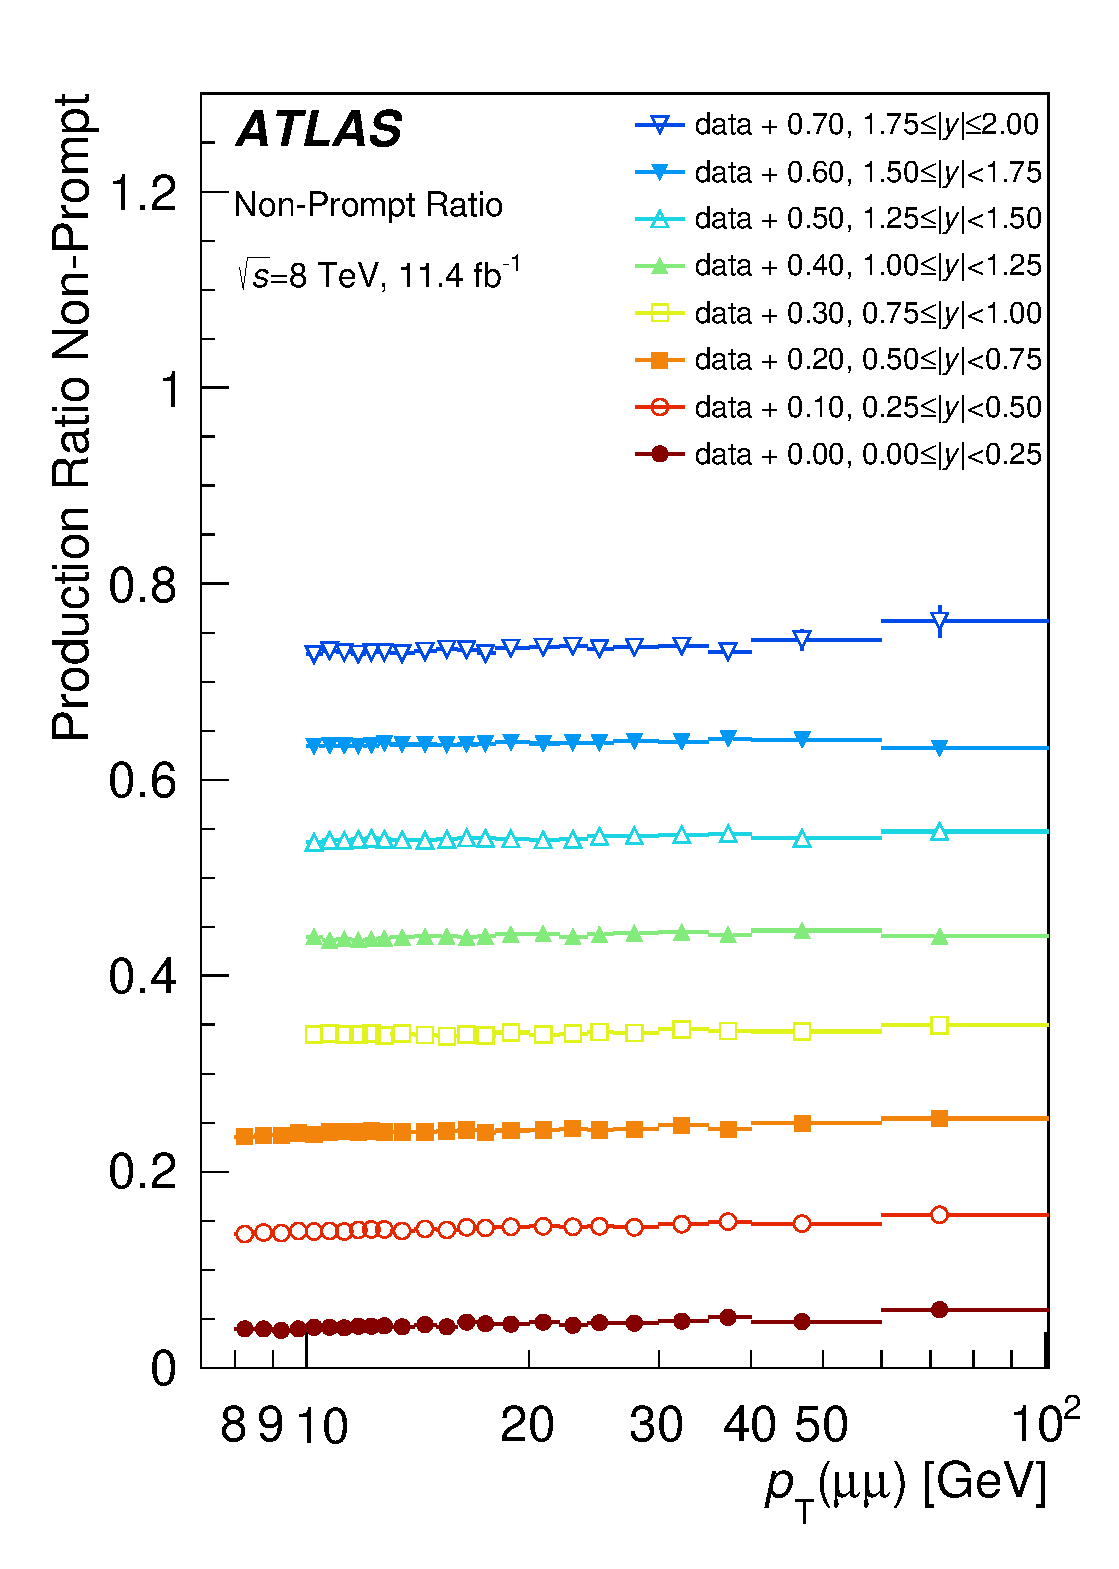
\includegraphics[width=0.44\textwidth]{figures/ct_8TeV_NP_Ratio.eps}\hfil
    \caption{The ratio of \psiprime\ to \jpsi\ production times dimuon branching fraction for prompt (left) and non-prompt (right) processes
    as a function of $\pt(\mu\mu)$  for each of the slices of rapidity. 
    For each increasing rapidity slice, an additional factor of 0.1 is applied to the plotted points for visual clarity.
    The top (bottom) row shows the 7~\TeV\ (8~\TeV) results.
      The centre of each bin on the horizontal axis represents the mean of the weighted $\pt$ distribution. The
      horizontal error bars represent the range of $\pt$ for the bin, and the vertical error bar covers the statistical and systematic uncertainty.}
    \label{fig:res:PNP_Ratio}
  \end{center}
\end{figure} 

\clearpage


\item[Comparison with theory] \hfill \\
For prompt production, as shown in Figure~\ref{fig:xsecPtheoryRatio}, the ratio of the NLO NRQCD theory calculations~\cite{Shao:2012iz} 
to data is provided for \Jpsi\ and \psiprime\ at both the 7 and 8~\TeV\ centre-of-mass energies.
The theory predictions are 
based on the long-distance matrix elements (LDMEs) from Refs.~\cite{NRQCD1,Ma:2010vd}, with uncertainties originating from the
choice of scale, charm quark mass and LDMEs (see Refs.~\cite{Shao:2012iz,Kanaki:2000ey,NRQCD1,Ma:2010vd} for more details).
Figure~\ref{fig:xsecPtheoryRatio} shows fair agreement between the theoretical calculation and the data points for the whole $\pt$ range. 
The ratio of theory to data does not depend on rapidity.

\begin{figure} [!ht]
  \begin{center}
    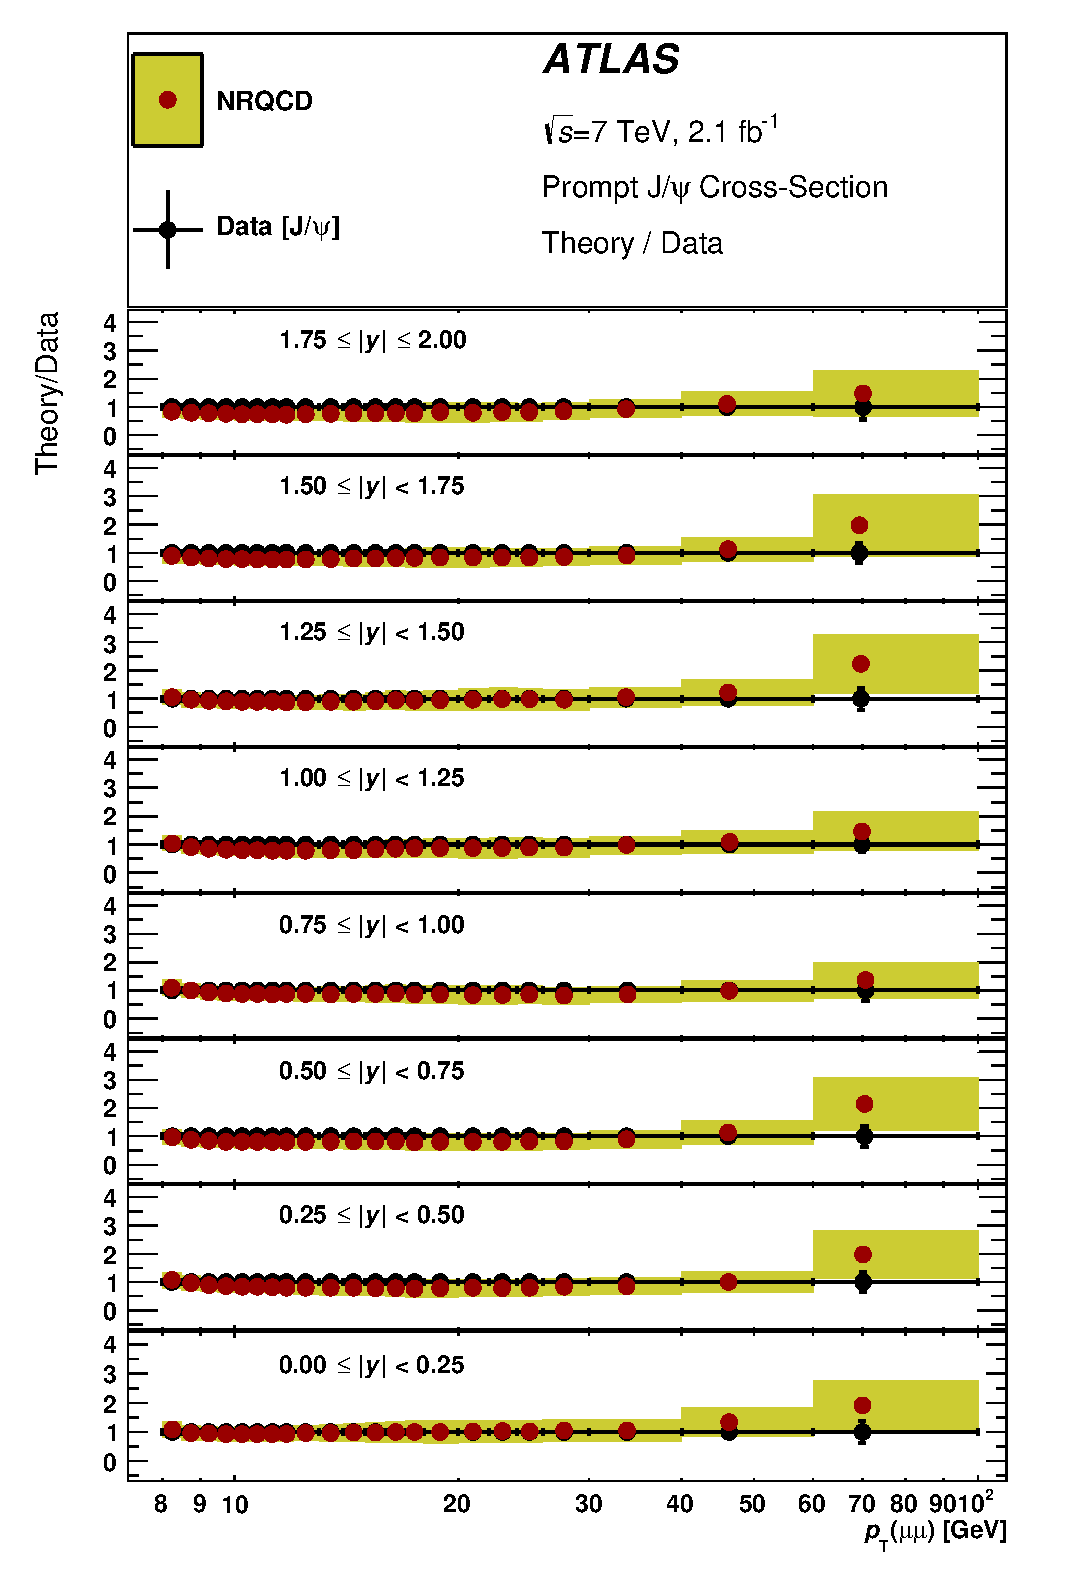
\includegraphics[width=0.44\textwidth]{figures/ct_7TeV_JpsiP_theoryRatio_lin.eps} 
    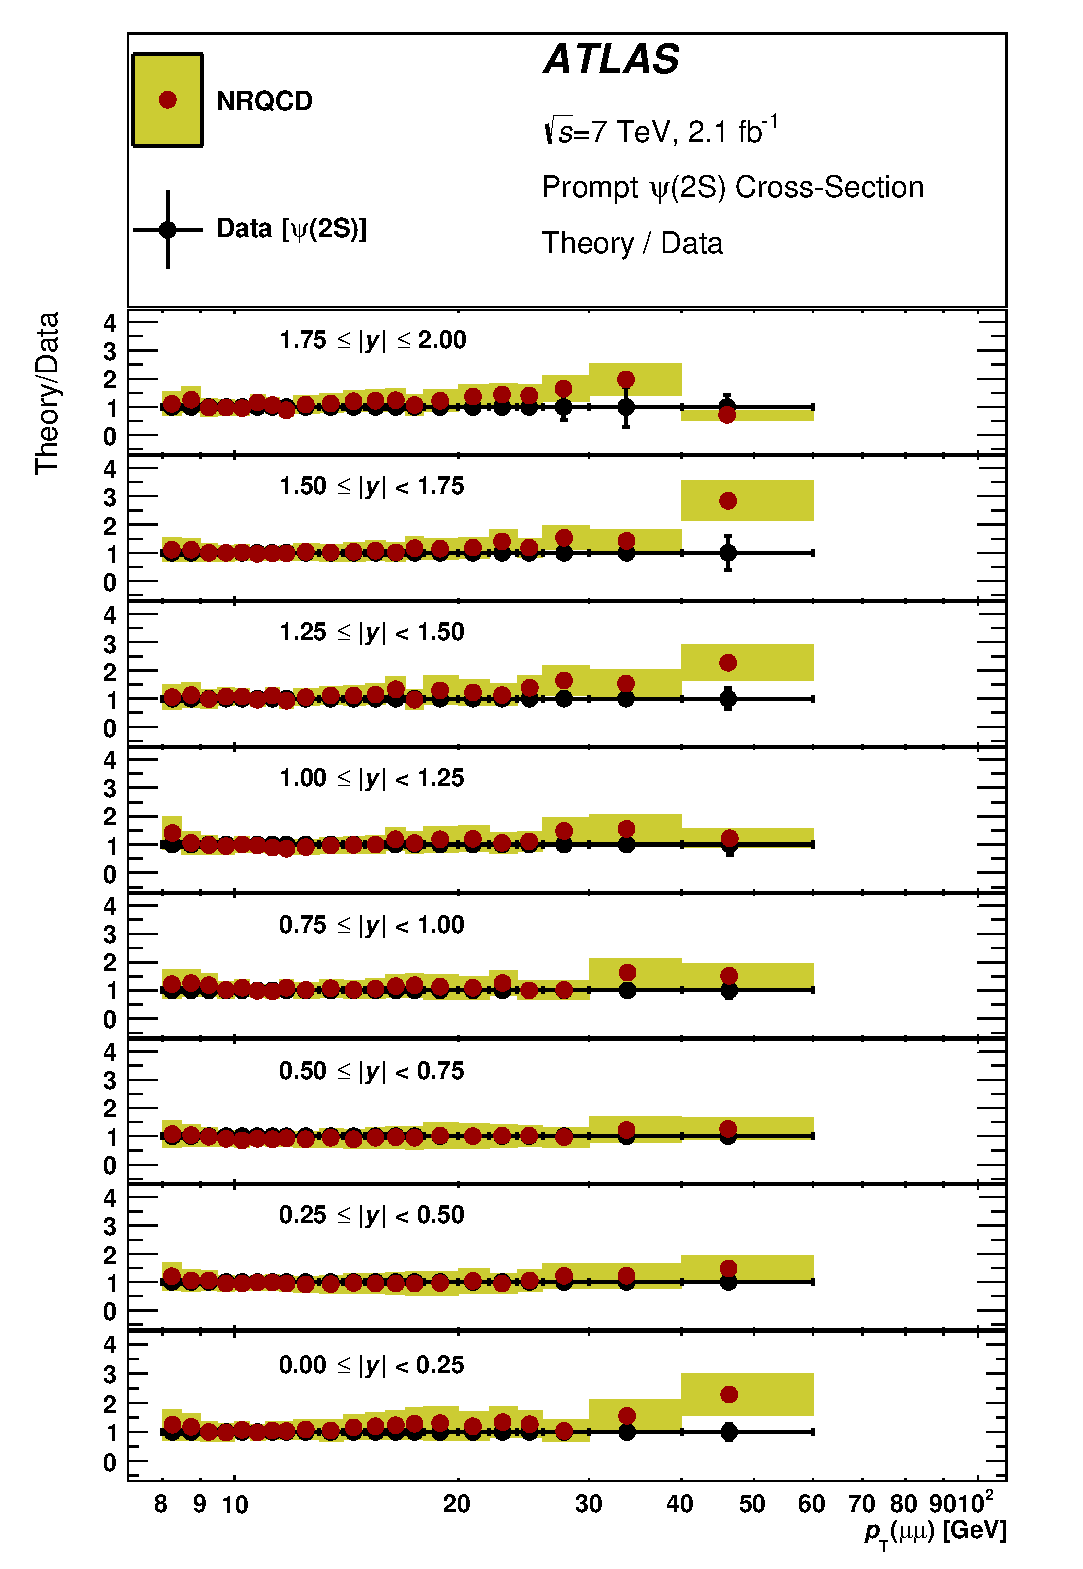
\includegraphics[width=0.44\textwidth]{figures/ct_7TeV_Psi2SP_theoryRatio_lin.eps}\hfil\\
    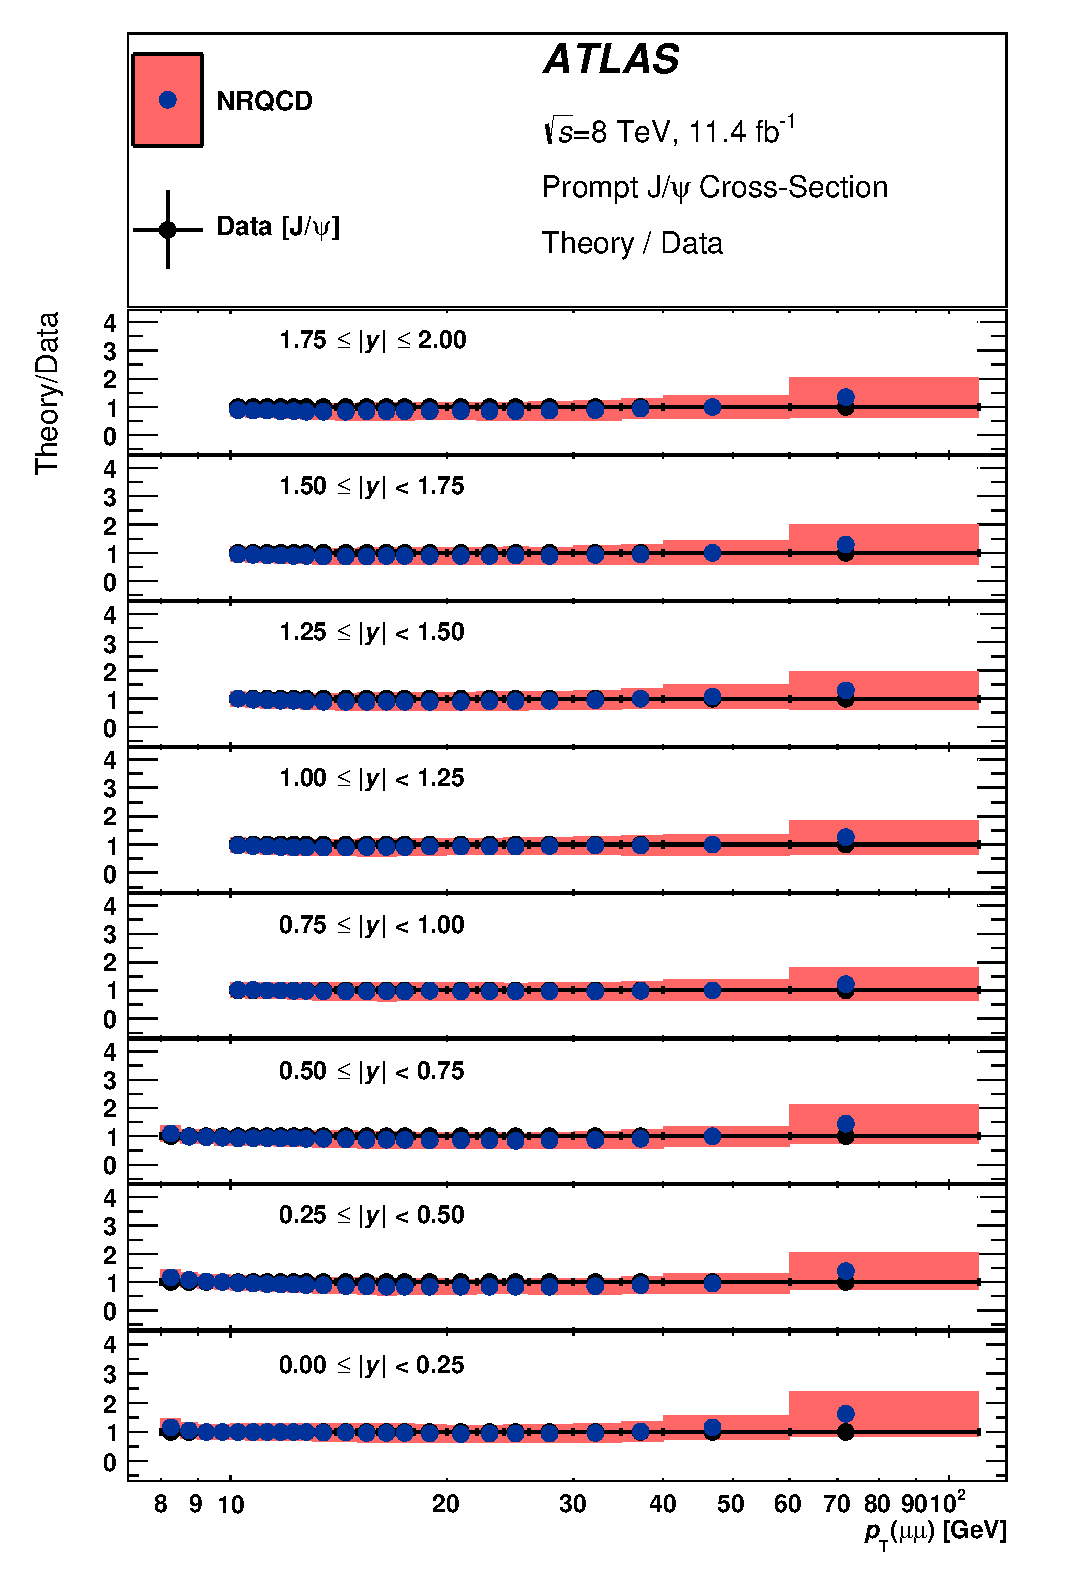
\includegraphics[width=0.44\textwidth]{figures/ct_8TeV_JpsiP_theoryRatio_lin.eps}
    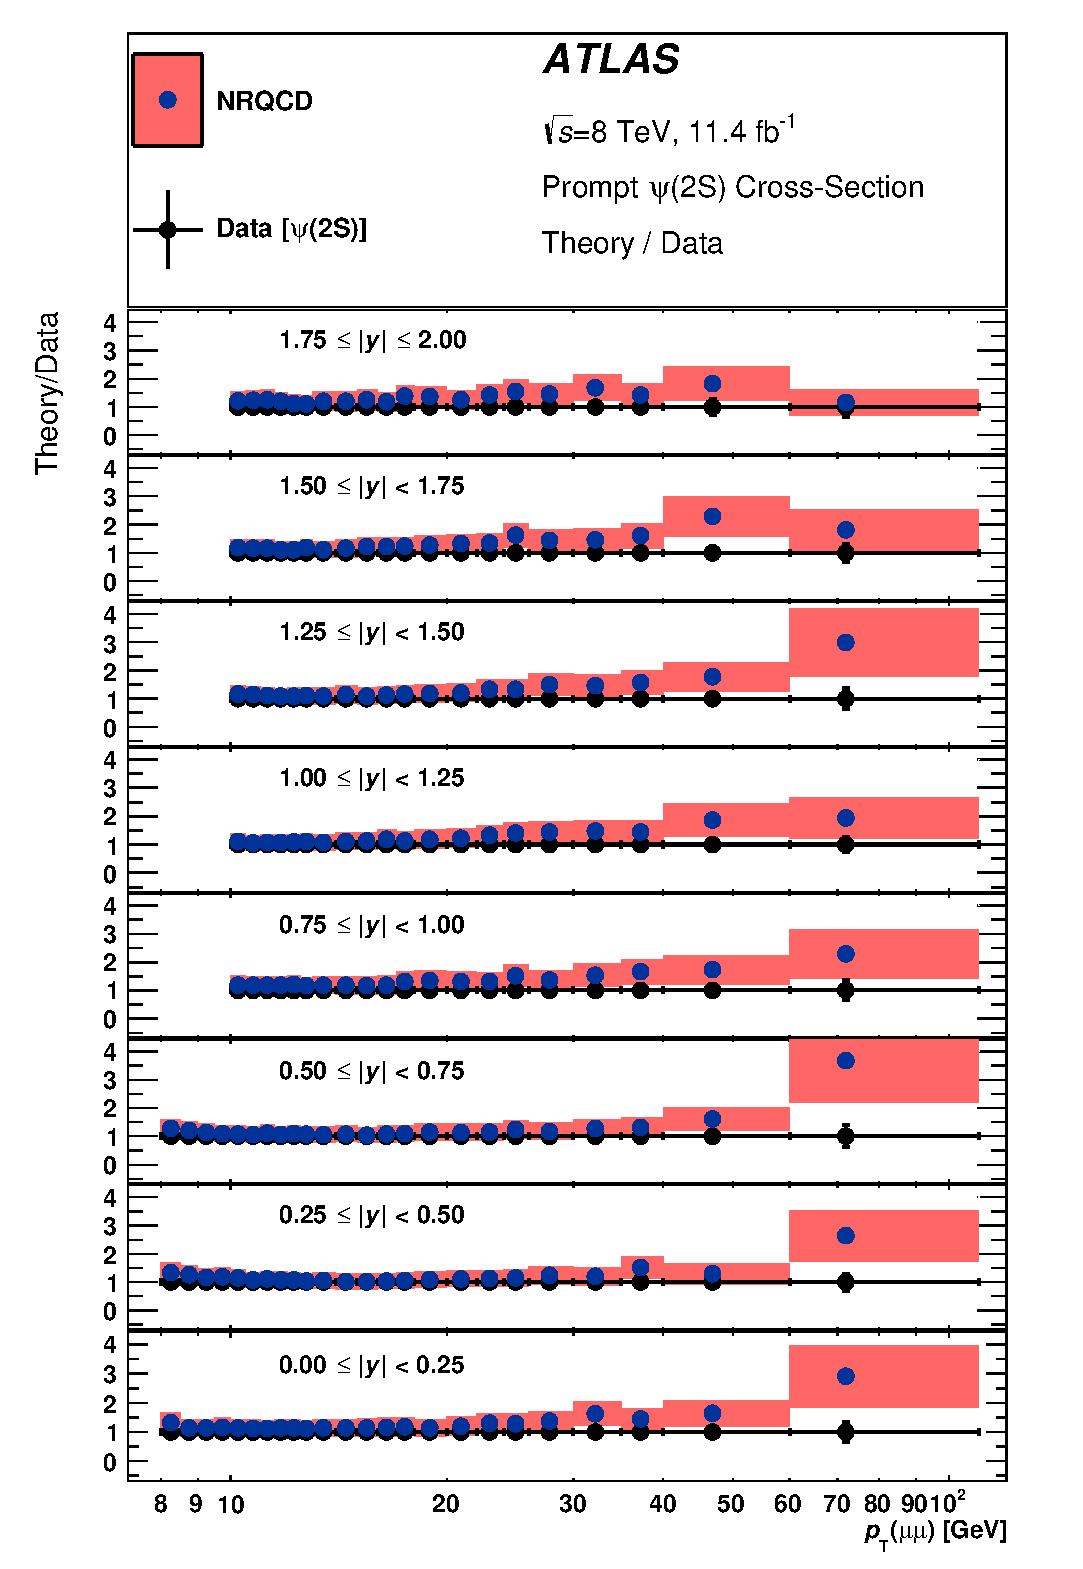
\includegraphics[width=0.44\textwidth]{figures/ct_8TeV_Psi2SP_theoryRatio_lin.eps}\hfil
    \caption{The ratios of the NRQCD theoretical predictions to data are presented for the differential prompt cross-section of \jpsi\ (left) and \psiprime\ (right) as a function 
    of $\pt(\mu\mu)$ for each rapidity slice. 
    The top (bottom) row shows the 7~\TeV\ (8~\TeV) results.
    The error on the data is the relative error of each data point, while the error bars on the theory prediction are the relative error of each theory point.}
    \label{fig:xsecPtheoryRatio}
  \end{center}
\end{figure} 

For non-prompt $\psi$ production, comparisons are made to FONLL theoretical predictions~\cite{FONLL_2001,Cacciari:2012ny}, which describe the production of 
$b$-hadrons followed by their decay into $\psi+X$.
Figure~\ref{fig:xsecNPtheoryRatio} shows the ratios of $\jpsi$ and $\psiprime$ FONLL predictions to data, as a function of $\pt$ and in slices of rapidity, 
for centre-of-mass energies of~7 and 8~\TeV.
For $\jpsi$, agreement is generally good, but the theory predicts slightly harder $\pt$ spectra than observed in the data.
For $\psiprime$, the shapes of data and theory appear to be in satisfactory agreement, but the theory predicts higher yields than in the data.
There is no observed dependence on rapidity in the comparisons between theory and data for non-prompt \jpsi\ and \psiprime\ production.


\begin{figure} [!ht]
  \begin{center}
    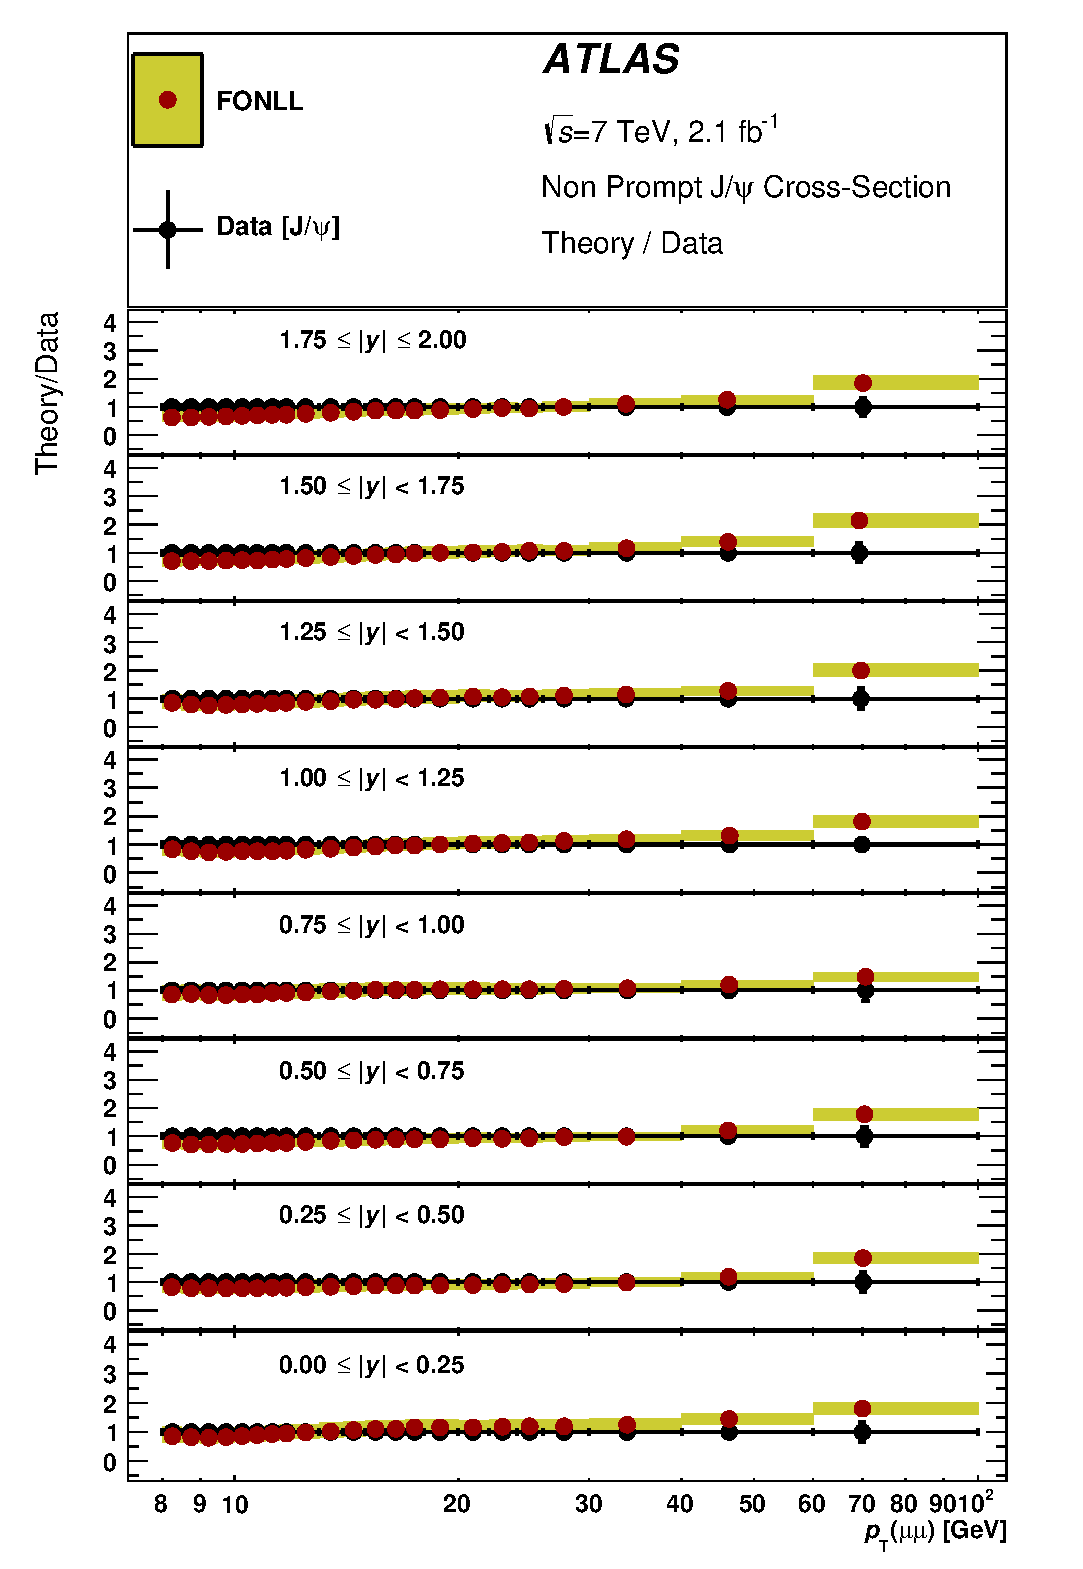
\includegraphics[width=0.44\textwidth]{figures/ct_7TeV_JpsiNP_theoryRatio_lin.eps} 
    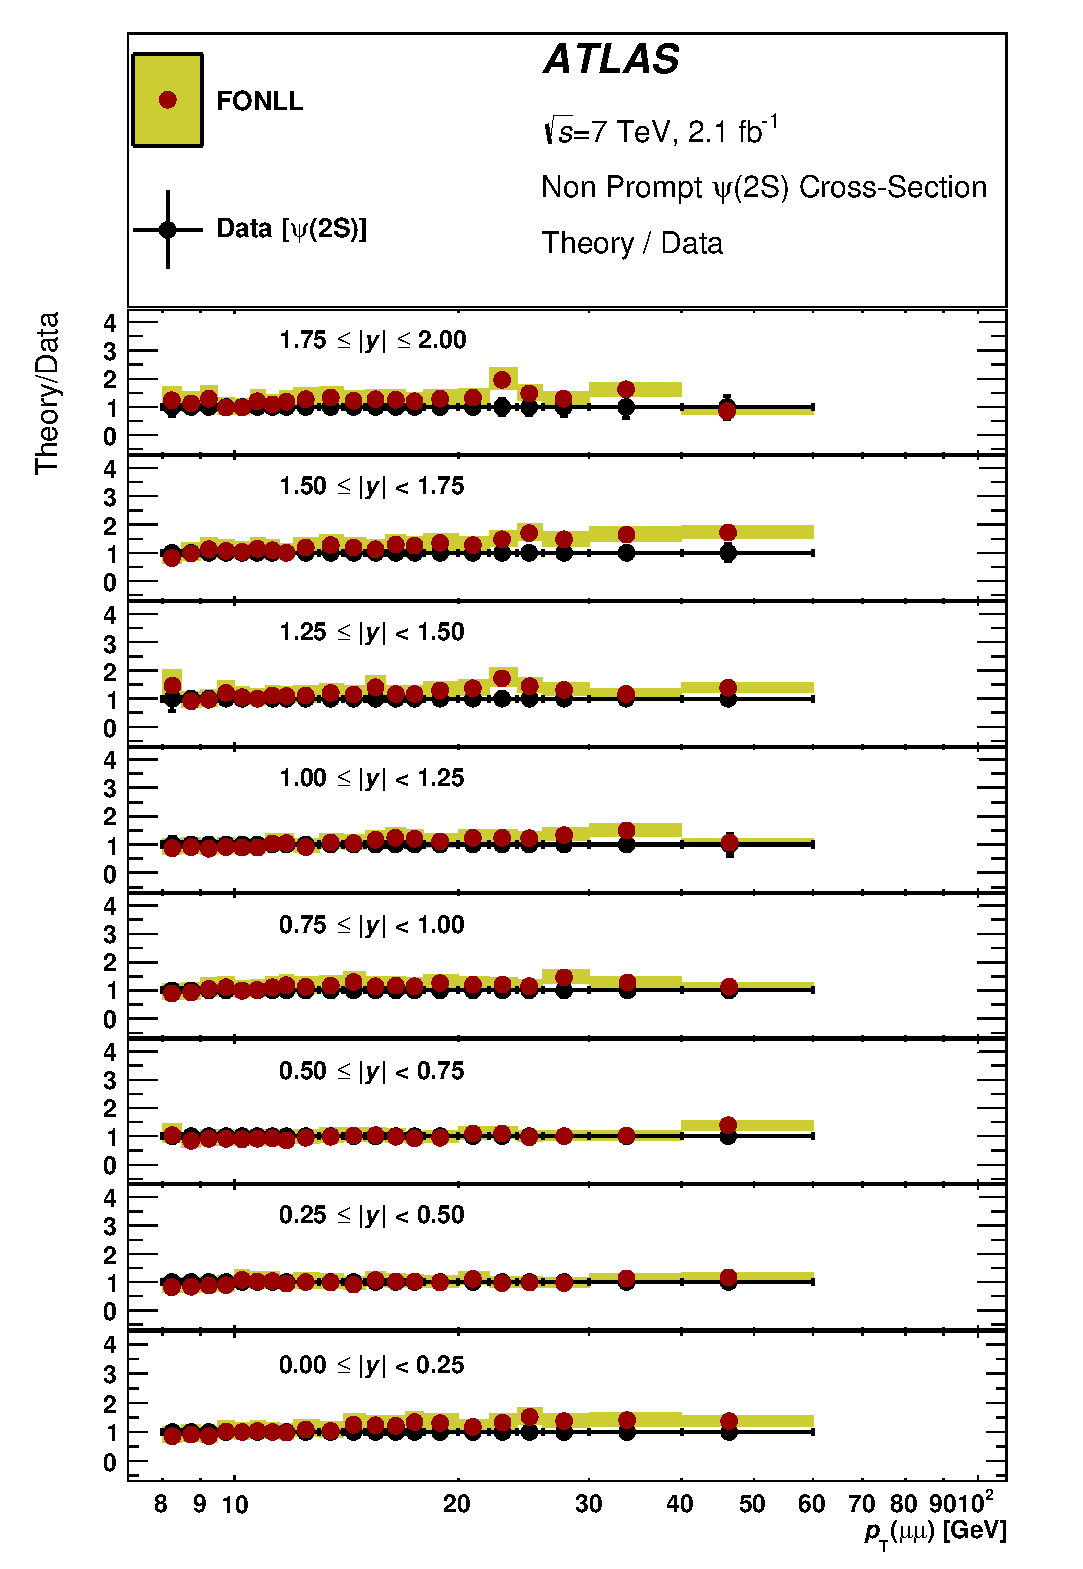
\includegraphics[width=0.44\textwidth]{figures/ct_7TeV_Psi2SNP_theoryRatio_lin.eps}\hfil\\
    \includegraphics[width=0.44\textwidth]{figures/ct_8TeV_JpsiNP_theoryRatio_lin.eps}
    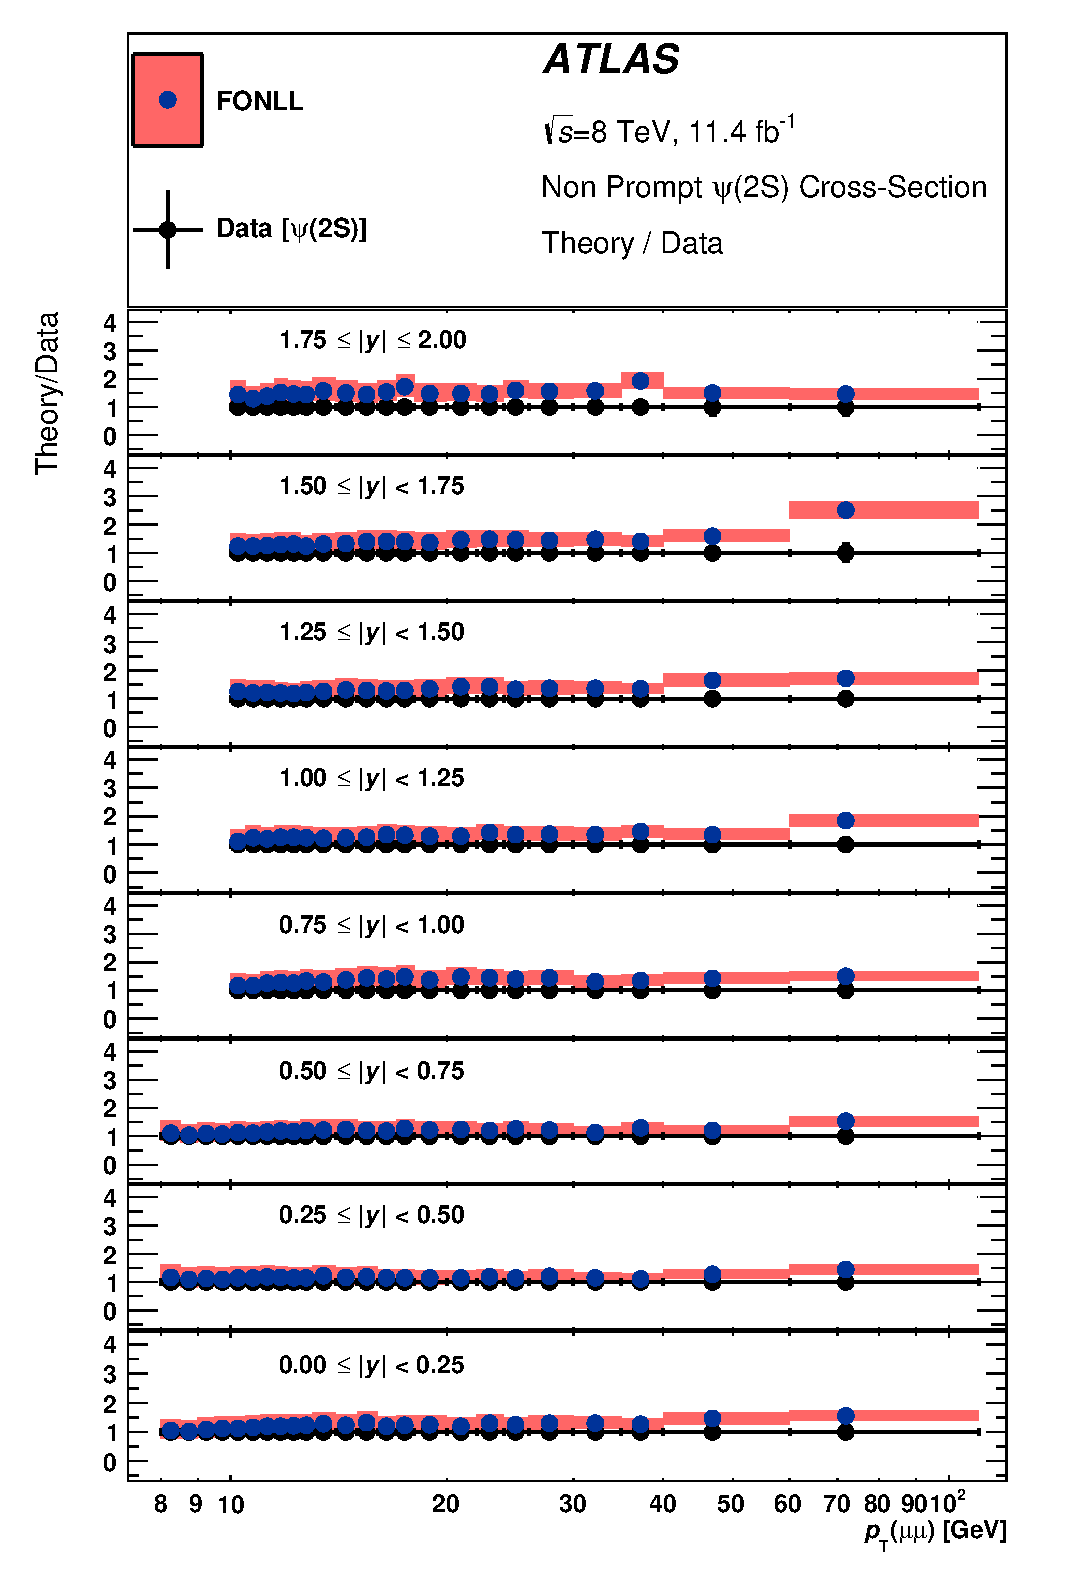
\includegraphics[width=0.44\textwidth]{figures/ct_8TeV_Psi2SNP_theoryRatio_lin.eps}\hfil
    \caption{The ratio of the FONLL theoretical predictions to data are presented for the differential non-prompt 
    cross-section of \jpsi\ (left) and \psiprime\ (right) as a function 
    of $\pt(\mu\mu)$ for each rapidity slice. 
    The top (bottom) row shows the 7~\TeV\ (8~\TeV) results.
    The error on the data is the relative error of each data point, while the error bars on the theory prediction are the relative error of each theory point.}
    \label{fig:xsecNPtheoryRatio}
  \end{center}
\end{figure} 


\item[Comparison of cross-sections 8~\TeV\  with 7~\TeV\ ] \hfill \\

It is interesting to compare the cross-section results between the two centre-of-mass energies, for both data and the theoretical predictions.

Figure~\ref{fig:xsecEnergyRatio} shows the 8~\TeV\  to 7~\TeV\  cross-section ratios of prompt and non-prompt $\jpsi$ and $\psiprime$ for both data sets.
For the theoretical ratios the uncertainties are neglected here, since the high correlation between them results in large cancellations.


Due to a finer granularity in $\pt$ for the 8~\TeV\  data, a weighted average of the 8~\TeV\ results is taken across equivalent intervals of the 7~\TeV\ data to enable direct comparisons.
Both data and theoretical predictions agree 
that the ratios become larger with increasing $\pt$,
however at the lower edge of the $\pT$ range the data tends to be slightly below theory.


\begin{figure} [!ht]
  \begin{center}
    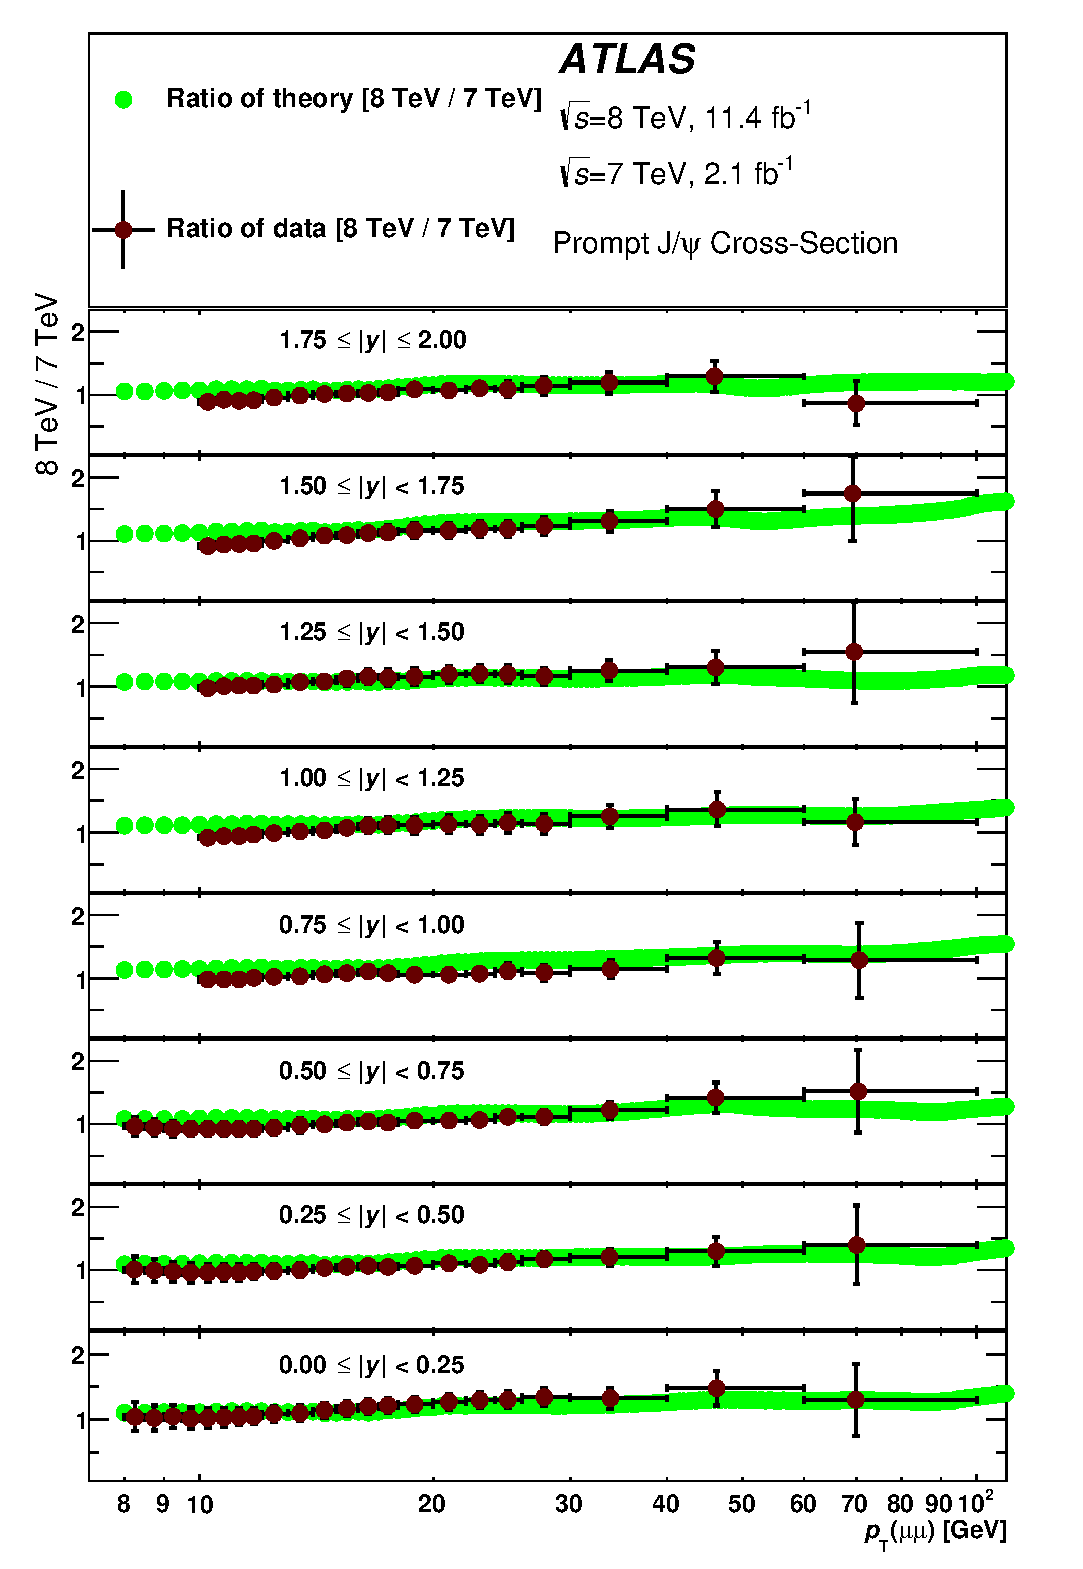
\includegraphics[width=0.44\textwidth]{figures/rt_th_xSecP_J.eps} 
    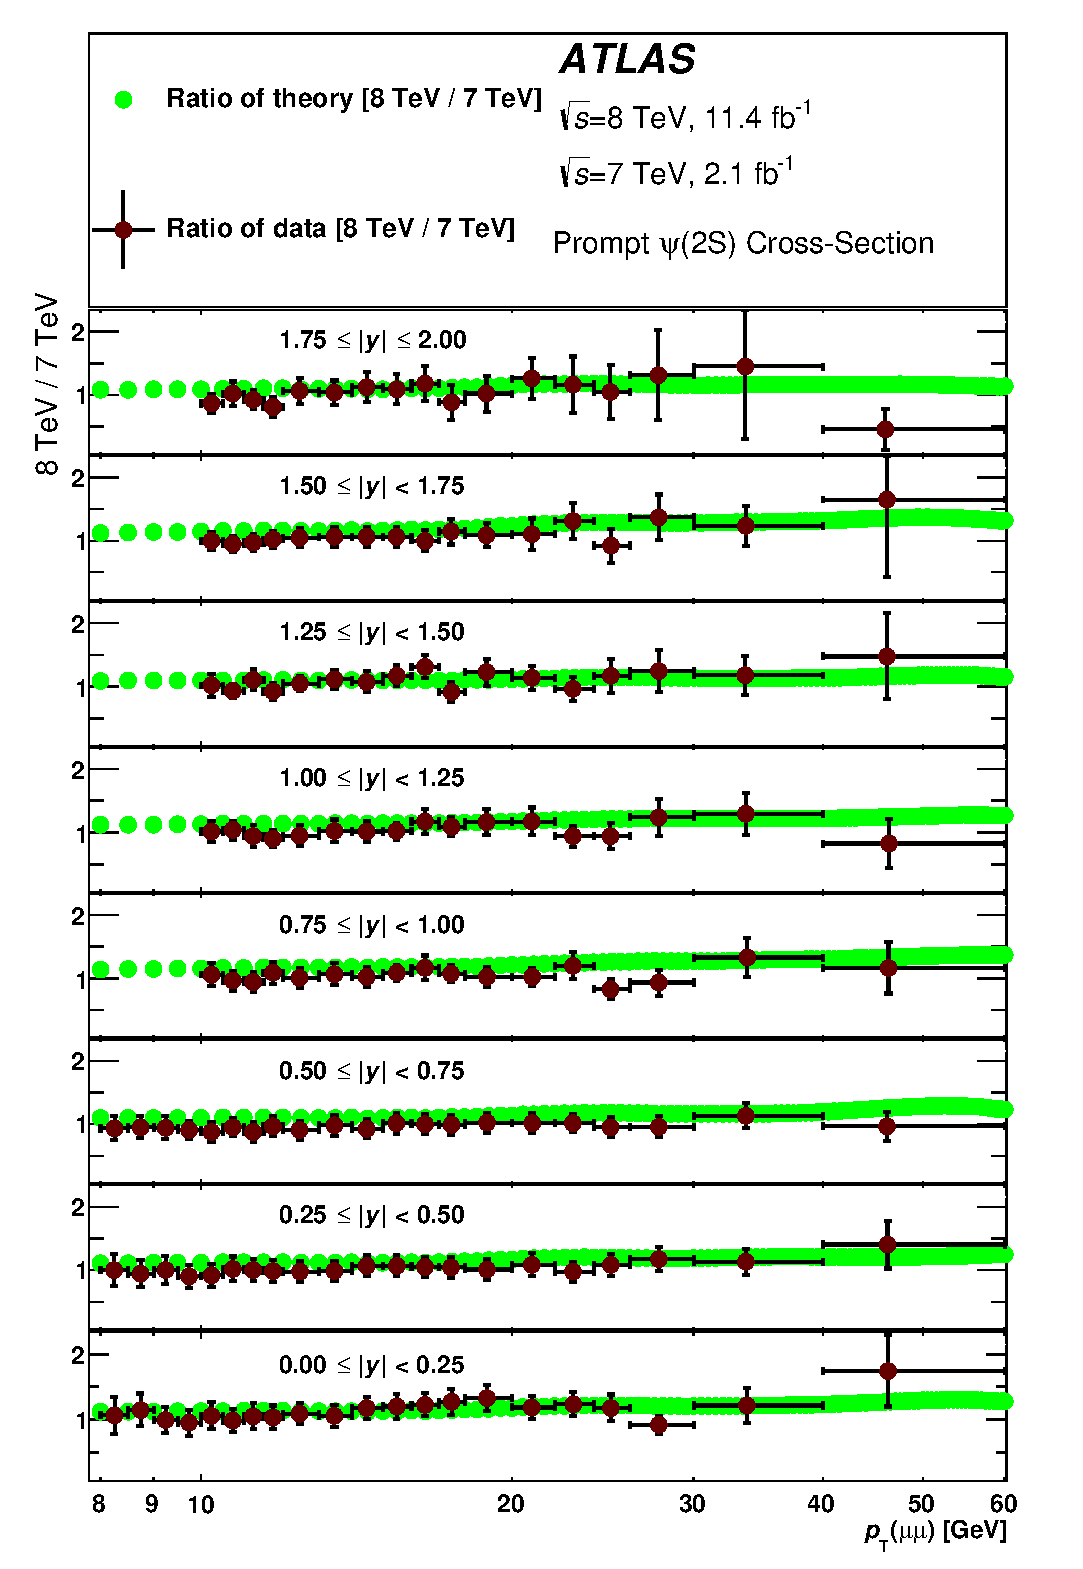
\includegraphics[width=0.44\textwidth]{figures/rt_th_xSecP_P.eps}\hfil\\
    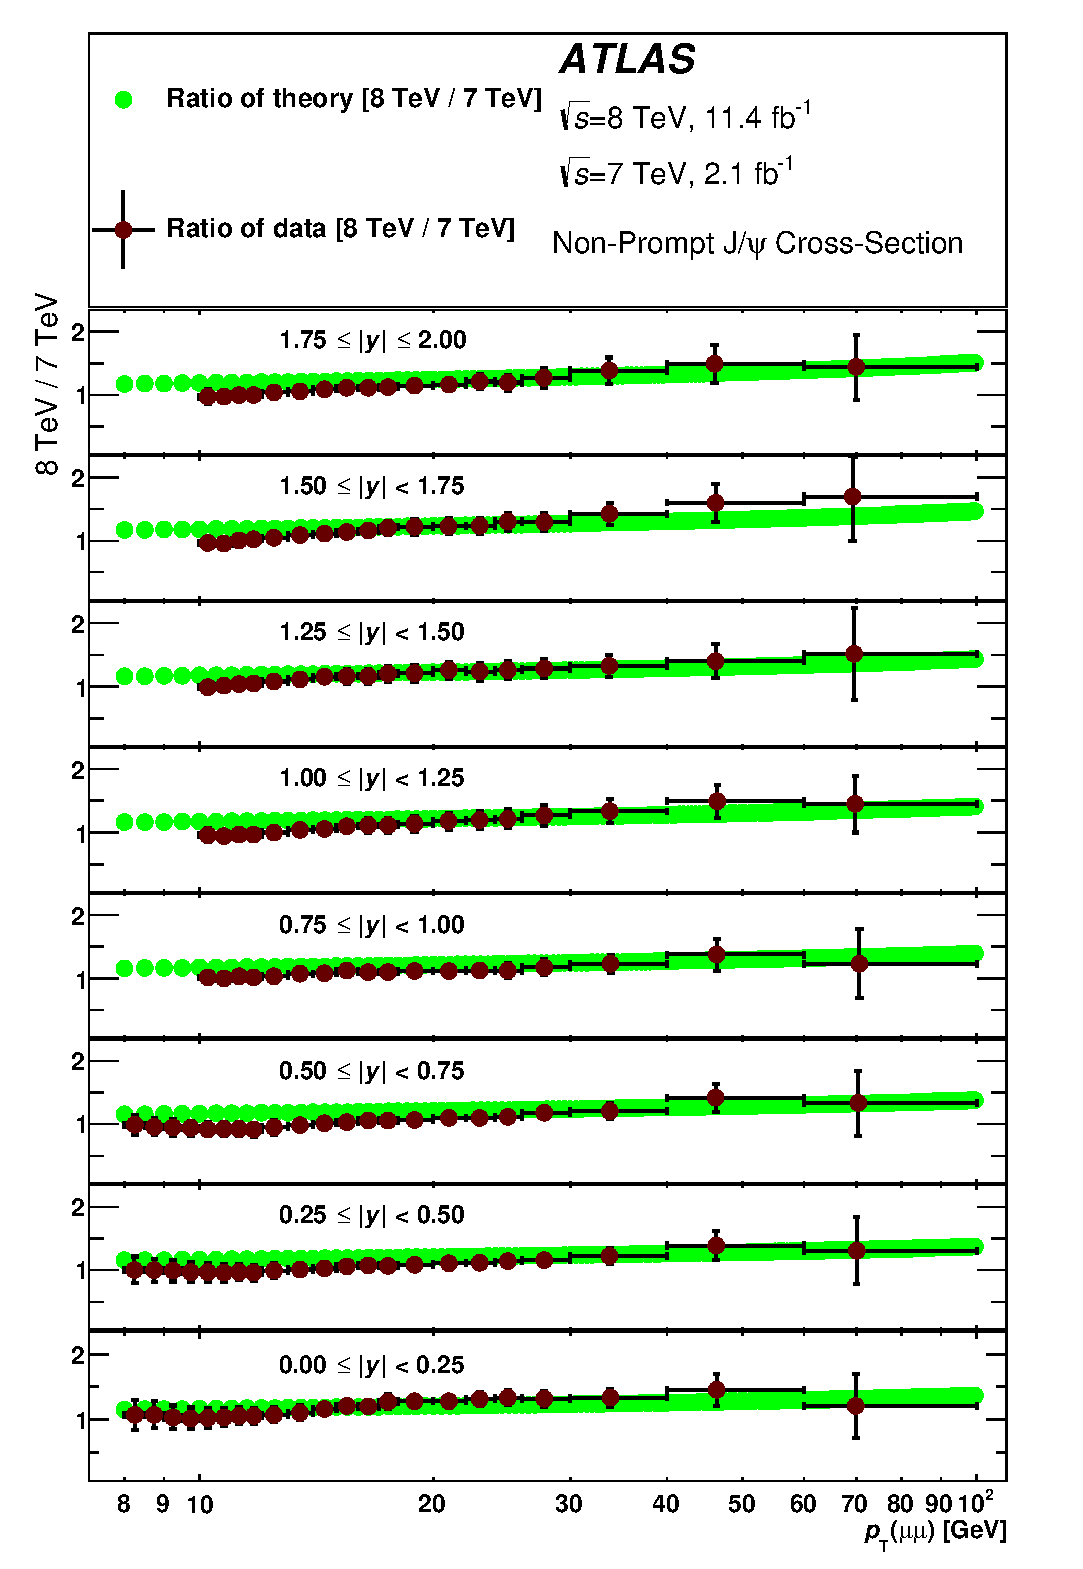
\includegraphics[width=0.44\textwidth]{figures/rt_th_xSecNP_J.eps}
    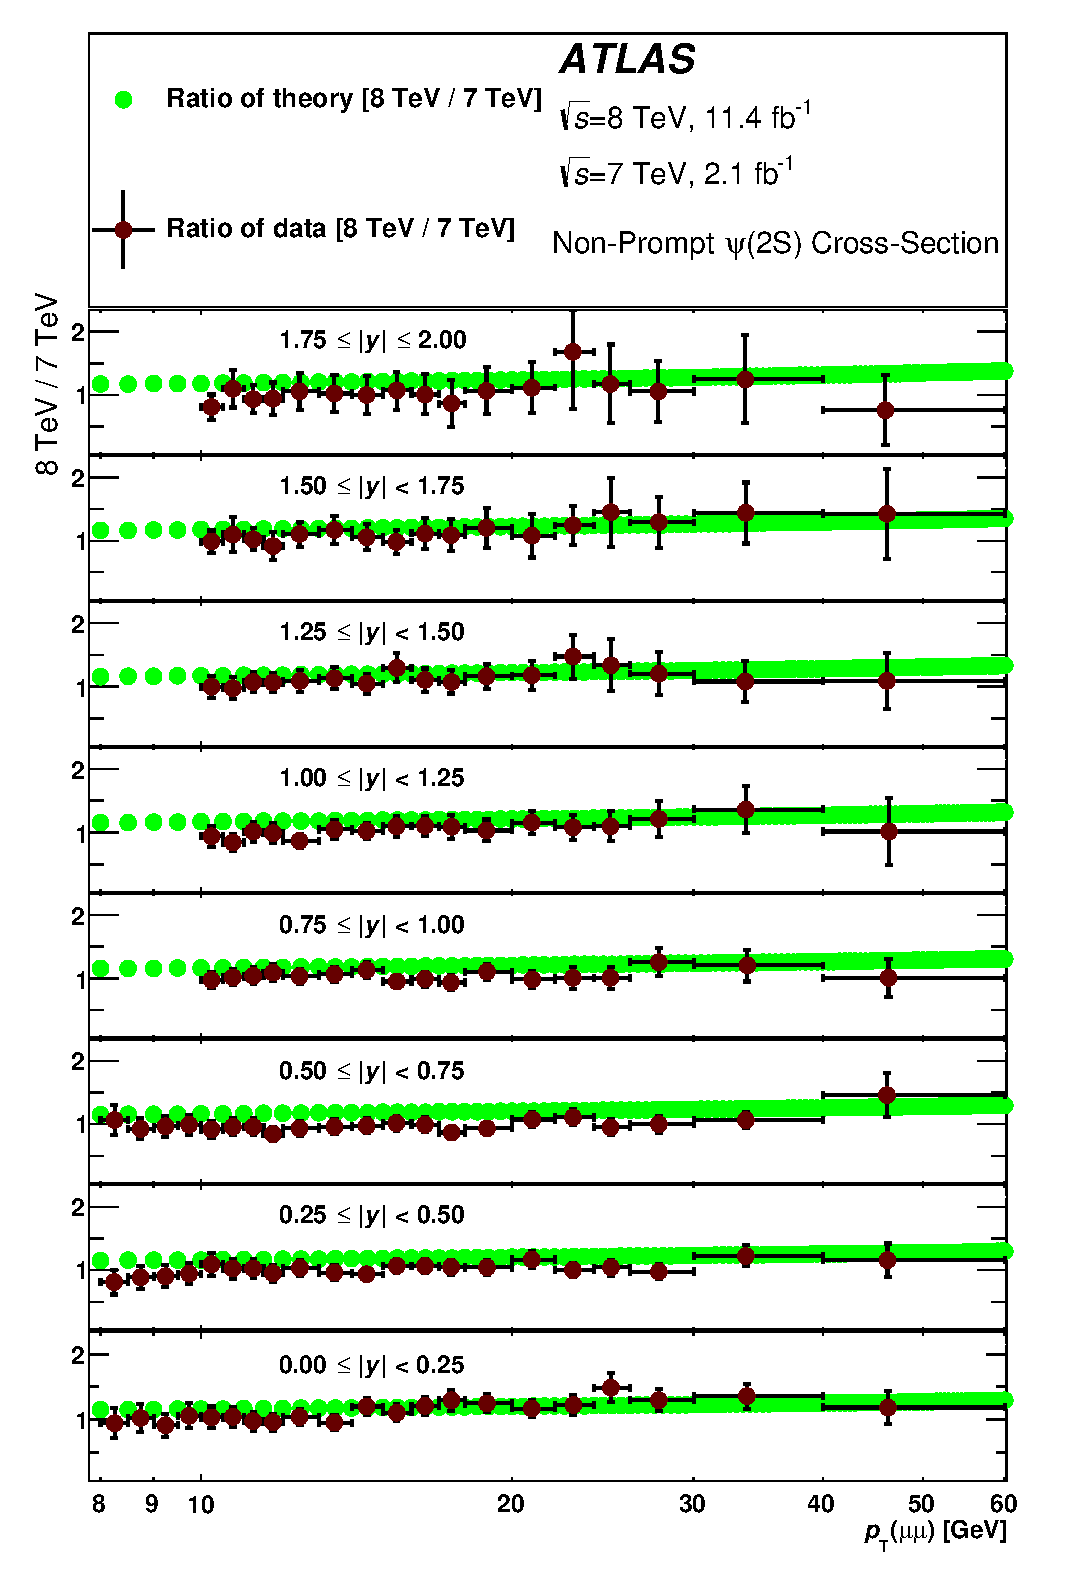
\includegraphics[width=0.44\textwidth]{figures/rt_th_xSecNP_P.eps}\hfil
    \caption{The ratio of the 8~\TeV\ and 7~\TeV\ differential cross-sections
	    are presented for prompt~(top) and non-prompt~(bottom) $\jpsi$~(left) and 
	    $\psiprime$~(right) for both data~(red points with error bars) and theoretical predictions~(green points).
	    The theoretical predictions used are NRQCD for prompt and FONLL for non-prompt production.
	    The uncertainty on the data ratio does not account for possible correlations between 7 and 8 \TeV\  data, and no uncertainty is shown 
	    for the ratio of theory predictions.
}
    \label{fig:xsecEnergyRatio}
  \end{center}
\end{figure} 


\end{description}
